\documentclass[aspectratio=169]{beamer}
\usepackage{will_handley_beamer}
\usepackage{title_page}
\usetikzlibrary{arrows,arrows.meta,automata,positioning}
\usepackage{slashed}

% Commands
% --------
% - \arxiv{arxiv number}
% - \arxiv{<number>}            arxiv.org/abs/<number>
% - \oldarxiv{<arxiv number>}   arxiv.org/<number>
% - \doi{<doi>}                 doi.org/<doi>
% - \xkcd{<number>}             xkcd.com/<number>
% - \email{<email>}             <<email>>
% - \tthref{<website>}          <website>
% - \av[dist]{<quantity>}       <quantity>_{dist}
% - \student{<name>}{<detail>}{<photo>}

% Talk details
% ------------
\title{ Nested sampling: {\large powering next-generation inference and machine learning tools}}
\subtitle{for astrophysics, cosmology, particle physics and beyond}
\date{30\textsuperscript{th} August 2024}

\begin{document}

\begin{frame}
    \titlepage
\end{frame}

\begin{frame}
    \frametitle{LBI: Likelihood-based inference}
    \begin{columns}
        \column{0.5\textwidth}
        The standard approach if you are fortunate enough to have a likelihood function $\only<1-2>{P(D|\theta)}\only<3->{\C[2]{\mathcal{L}(D|\theta)}}$: 
        \[
            \only<1-2>{
                P(\theta|D) = \frac{P(D|\theta)P(\theta)}{P(D)}
            }
            \only<2>{
                \qquad
                \C[0]{\text{Posterior}} = \frac{\C[2]{\text{Likelihood}}\times\C[1]{\text{Prior}}}{\C[3]{\text{Evidence}}}
            }
            \only<3>{
                \C[0]{\mathcal{P}(\theta|D)} = \frac{\C[2]{\mathcal{L}(D|\theta)}\C[1]{\pi(\theta)}}{\C[3]{\mathcal{Z}(D)}}
                \qquad
                \C[0]{\text{Posterior}} = \frac{\C[2]{\text{Likelihood}}\times\C[1]{\text{Prior}}}{\C[3]{\text{Evidence}}}
            }
            \only<4>{
                P(\theta|D) P(D) = P(\theta,D) = P(D|\theta)P(\theta), \qquad
            }
            \only<5>{
                \C[0]{\mathcal{P}}\times\C[3]{\mathcal{Z}} = \C[4]{\mathcal{J}} = \C[2]{\mathcal{L}}\times\C[1]{\pi}, \qquad \C[4]{\text{Joint}} = \C[4]{\mathcal{J}} = P(\theta,D)
            }
        \]
        \vspace{-10pt}
        \begin{enumerate}
            \item Define \C[1]{prior $\pi(\theta)$} 
                \begin{itemize}
                    \item spend some time being philosophical
                \end{itemize}
            \item Sample \C[0]{posterior $\mathcal{P}(\theta|D)$} 
                \begin{itemize}
                    \item use out-of-the-box MCMC tools such as\\ \texttt{emcee} or \texttt{MultiNest}
                    \item make some triangle plots
                \end{itemize}
            \item Optionally compute \C[3]{evidence $\mathcal{Z}(D)$}
                \begin{itemize}
                    \item e.g. nested sampling or parallel tempering
                    \item do some model comparison (i.e. science)
                    \item talk about tensions
                \end{itemize}
        \end{enumerate}
        \column{0.5\textwidth}
        \hfill%
        \begin{overpic}[width=0.6\textwidth]{figures/des_parameters.pdf}
            \put(-40,90) {DES Y5 SN Ia}
            \put(-40,80) {\arxiv{2401.02929}}
        \end{overpic}
        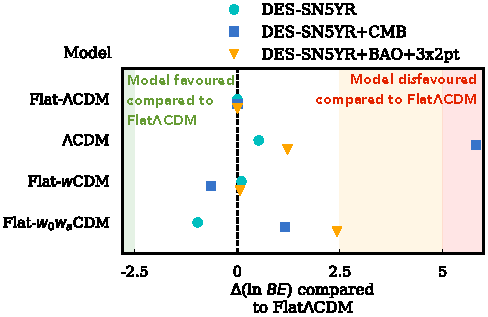
\includegraphics[width=0.5\textwidth]{figures/des_model_comparison.pdf}%
        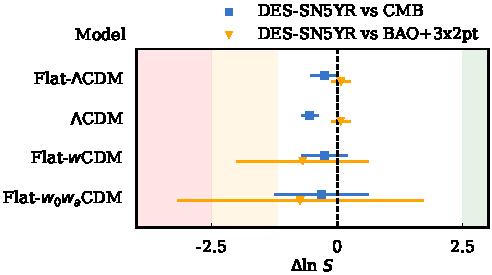
\includegraphics[width=0.5\textwidth]{figures/des_suspiciousness.pdf}
    \end{columns}
\end{frame}

\begin{frame}
    \frametitle{The three pillars of Bayesian inference}
    \begin{columns}[t]
        \column{0.33\textwidth}
        \begin{block}{Parameter estimation}
            What do the data tell us about the parameters of a model?\\
            \textit{e.g. the size or age of a $\Lambda$CDM universe}
            \[ \hspace{-4pt}\C[0]{P(\theta|D,M)} = \frac{\C[2]{P(D|\theta,M)} \C[1]{P(\theta|M)}}{\C[3]{P(D|M)}} \] 
            \[ \C[0]{\mathcal{P}} = \frac{\C[2]{\mathcal{L}} \times\C[1]{\pi}}{\C[3]{\mathcal{Z}}}\] 
            \[ \C[0]{\text{Posterior}} = \frac{\C[2]{\text{Likelihood}} \times\C[1]{\text{Prior}}}{\C[3]{\text{Evidence}}}\]
        \end{block}
        \column{0.3\textwidth}
        \begin{block}{Model comparison}
            How much does the data support a particular model?\\
            \textit{e.g. $\Lambda$CDM vs a dynamic dark energy cosmology}
            \[ \C[4]{P(M|D)} = \frac{\C[3]{P(D|M)} \C[5]{P(M)}}{\C[7]{P(D)}} \vspace{-7pt}\]
            \[ \frac{\C[3]{\mathcal{Z}_{M}} \C[5]{\Pi_{M}}}{\C[7]{\sum_m Z_m \Pi_m}} \]
            \[ \C[4]{\text{Posterior}} = \frac{\C[3]{\text{Evidence}} \times\C[5]{\text{Prior}}}{\C[7]{\text{Normalisation}}}\]
        \end{block}
        \column{0.33\textwidth}
        \begin{block}{Tension quantification}
            Do different datasets make consistent predictions from the same model? 
            \textit{e.g. CMB vs Type IA supernovae data}
            \[ \mathcal{R} = \frac{\C[3]{\mathcal{Z}}_{AB}}{\C[3]{\mathcal{Z}}_A\C[3]{\mathcal{Z}}_\mathcal{B}}\] 
            \[
                \begin{aligned} \log\mathcal{S} = \av[{\C[0]{\mathcal{P}}_{AB}}]{\C[2]{\log\mathcal{L}}_{AB}}&\\
                    -\av[{\C[0]{\mathcal{P}}_{A}}]{\C[2]{\log\mathcal{L}}_{A}}&\\
                    -\av[{\C[0]{\mathcal{P}}_{B}}]{\C[2]{\log\mathcal{L}}_{B}}&
                \end{aligned}
            \]
        \end{block}
    \end{columns}
\end{frame}

\begin{frame}
    \frametitle{Model comparison $\C[3]{\mathcal{Z}=P(D|M)}$}
    \begin{itemize}
        \item Bayesian model comparison allows mathematical derivation of key philosophical principles.
    \end{itemize}
    \begin{columns}[t]
        \column{0.47\textwidth}
        Viewed from data-space $D$:
        \begin{block}{Popper's falsificationism}
            \begin{itemize}
                \item Prefer models that make bold predictions.
                \item if proven true, model more likely correct.
            \end{itemize}
        \end{block}
        \includegraphics<1|handout:0>[width=\textwidth, page=1]{figures/popper}%
        \includegraphics<2|handout:0>[width=\textwidth, page=2]{figures/popper}%
        \includegraphics<3>[width=\textwidth, page=3]{figures/popper}%
        \begin{itemize}
            \item Falsificationism comes from normalisation
        \end{itemize}
        \column{0.47\textwidth}
        Viewed from parameter-space $\theta$:
        \begin{block}{Occam's razor}
            \begin{itemize}
                \item Models should be as simple as possible
                \item \ldots but no simpler
            \end{itemize}
        \end{block}
        \begin{itemize}
            \item Occam's razor equation:
                \[\C[3]{\log\mathcal{Z}} = \av[{\C[0]{\mathcal{P}}}]{\C[2]{\log\mathcal{L}}} - \mathcal{D}_\text{KL}\]
            \item ``Occam penalty'': KL divergence between \C[1]{prior~$\pi$} and \C[0]{posterior~$\mathcal{P}$}.
                \[ \mathcal{D}_\text{KL}\sim \log\frac{\text{\C[1]{Prior volume} }}{\text{\C[0]{Posterior volume}}}\]
        \end{itemize}
    \end{columns}
\end{frame}

\begin{frame}
    \frametitle{What is Nested Sampling?}
    \begin{itemize}
        \item Nested sampling is a radical, multi-purpose numerical tool.
        \item Given a (scalar) function $f$ with a vector of parameters $\theta$, it can be used for:
    \end{itemize}
    \vspace{-10pt}
    \begin{columns}[t]
        \column{0.3\textwidth}
        \begin{block}{Optimisation}
            \[\theta_\text{max} = \max_\theta{f(\theta)}\]
        \end{block}
        \column{0.3\textwidth}
        \begin{block}{Exploration}
            \vspace{-10pt}
            \[\text{draw/sample}\quad \theta\sim f\]
            \vspace{-15pt}
        \end{block}
        \column{0.3\textwidth}
        \begin{block}{Integration}
            \[\int f(\theta) dV \]
        \end{block}
    \end{columns}
    \begin{columns}[t]
        \column{0.33\textwidth}
        \centerline{\includegraphics[width=0.8\textwidth,page=13]{figures/himmelblau}}
        \column{0.33\textwidth}
        \centerline{\includegraphics[width=0.8\textwidth,page=15]{figures/himmelblau}}
        \column{0.33\textwidth}
        \centerline{\includegraphics[width=0.8\textwidth,page=14]{figures/himmelblau}}
    \end{columns}
\end{frame}

\begin{frame}
    \frametitle{Where is Nested Sampling?}
    \begin{columns}
        \column{0.5\textwidth}
        \begin{itemize}
            \item For many purposes, in your Neural Net you should group Nested Sampling with (MCMC) techniques such as:
                \begin{itemize}
                    \item Metropolis-Hastings (PyMC, MontePython)
                    \item Hamiltonian Monte Carlo (Stan, blackjax)
                    \item Ensemble sampling (emcee, zeus). 
                    \item Variational Inference (Pyro)
                    \item Sequential Monte Carlo 
                    \item Thermodynamic integration
                    \item Genetic algorithms
                \end{itemize}
            \item You may have heard of it branded form:
                \begin{itemize}
                    \item MultiNest
                    \item PolyChord
                    \item dynesty
                    \item ultranest
                \end{itemize}
            \end{itemize}
        \column{0.5\textwidth}
        \begin{columns}
            \column{0.5\textwidth}
        \includegraphics[width=\textwidth]{figures/emcee}
        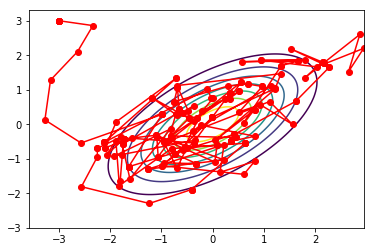
\includegraphics[width=\textwidth]{figures/metropolis-hastings}
            \column{0.5\textwidth}
        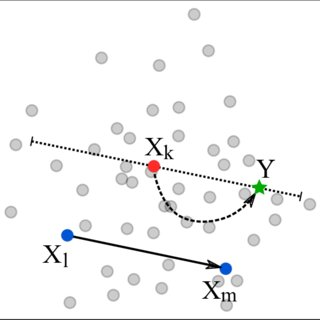
\includegraphics[width=\textwidth]{figures/zeus}
        \end{columns}
        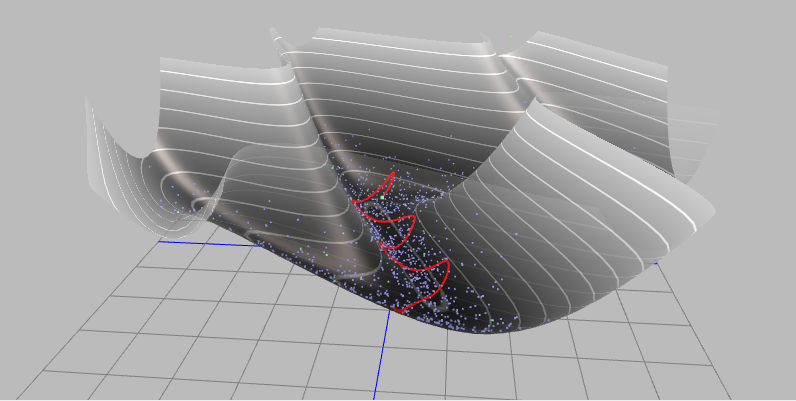
\includegraphics[width=\textwidth]{figures/hmc_explained}
    \end{columns}
\end{frame}

\begin{frame}
    \frametitle{Integration in Physics}
    \begin{itemize}
        \item Integration is a fundamental concept in physics, statistics and data science:
    \end{itemize}
    \begin{columns}
        \column{0.3\textwidth}
        \begin{block}{Partition functions}
            \vspace{-11pt}
            \[ Z(\beta) = \int e^{-\beta H(q,p)} dq dp \]
        \end{block}
        \column{0.3\textwidth}
        \begin{block}{Path integrals}
            \[ \Psi = \int e^{i S} \mathcal{D}x \]
        \end{block}
        \column{0.3\textwidth}
        \begin{block}{Bayesian marginals}
            \vspace{-11pt}
            \[ \mathcal{Z}(D) = \int \mathcal{L}(D|\theta) \pi(\theta) d\theta \]
        \end{block}
    \end{columns}
    \begin{columns}
        \column{0.6\textwidth}
        \begin{itemize}
            \item Need numerical tools if analytic solution unavailable.
            \item High-dimensional numerical integration is hard.
            \item Riemannian strategy estimates volumes geometrically:
                \[ \int f(x) d^nx \approx \sum_i f(x_i) \Delta V_i \sim \mathcal{O}(e^n) \]
            \item Curse of dimensionality $\Rightarrow$ exponential scaling.
        \end{itemize}
        \column{0.4\textwidth}
        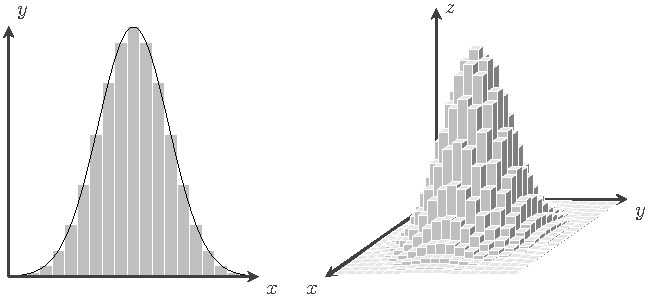
\includegraphics[width=\textwidth]{figures/integration.pdf}
    \end{columns}
\end{frame}

\begin{frame}
    \begin{columns}
        \column{0.48\textwidth}
        \begin{block}{\textbf{MCMC}}
            \only<16>{
                \begin{itemize}
                    \item Single ``walker''
                    \item Explores posterior
                    \item Fast, if proposal matrix is tuned
                    \item Parameter estimation, suspiciousness calculation
                    \item Channel capacity optimised for generating posterior samples
                \end{itemize}
            }
        \end{block}
            \includegraphics<1>[width=\textwidth,page=16]{figures/himmelblau}%
            \includegraphics<2>[width=\textwidth,page=17]{figures/himmelblau}%
            \includegraphics<3>[width=\textwidth,page=18]{figures/himmelblau}%
            \includegraphics<4>[width=\textwidth,page=19]{figures/himmelblau}%
            \includegraphics<5>[width=\textwidth,page=20]{figures/himmelblau}%
            \includegraphics<6-15>[width=\textwidth,page=21]{figures/himmelblau}%
        \centerline{\includegraphics<16>[width=0.5\textwidth,page=19]{figures/himmelblau}}
        \column{0.48\textwidth}
        \begin{block}<7->{\textbf{Nested sampling}}
            \only<16>{
                \begin{itemize}
                    \item Ensemble of ``live points''
                    \item Scans from prior to peak of likelihood
                    \item Slower, no tuning required
                    \item Parameter estimation, model comparison, tension quantification
                    \item Channel capacity optimised for computing partition function
                \end{itemize}
            }
        \end{block}
            \includegraphics<7|handout:0>[width=\textwidth,page=1]{figures/himmelblau}%
            \includegraphics<8|handout:0>[width=\textwidth,page=2]{figures/himmelblau}%
            \includegraphics<9|handout:0>[width=\textwidth,page=3]{figures/himmelblau}%
            \includegraphics<10          >[width=\textwidth,page=4]{figures/himmelblau}%
            \includegraphics<11|handout:0>[width=\textwidth,page=5]{figures/himmelblau}%
            \includegraphics<12|handout:0>[width=\textwidth,page=6]{figures/himmelblau}%
            \includegraphics<13|handout:0>[width=\textwidth,page=7]{figures/himmelblau}%
            \includegraphics<14|handout:0>[width=\textwidth,page=8]{figures/himmelblau}%
            \includegraphics<15|handout:0>[width=\textwidth,page=15]{figures/himmelblau}%
        \centerline{\includegraphics<16>[width=0.5\textwidth,page=4]{figures/himmelblau}} 
    \end{columns}
\end{frame}

\begin{frame}
    \frametitle{The nested sampling meta-algorithm: live points}
    \begin{columns}
        \column{0.5\textwidth}
        \begin{itemize}
            \item Start with $n$ random samples over the space.
            \item Delete outermost sample, and replace with a new random one at higher integrand value.
            \item The ``live points'' steadily contract around the peak(s) of the function.
            \item We can use this evolution to estimate volume \emph{probabilistically}.
            \item At each iteration, the contours contract by $\sim\frac{1}{n}\only<5->{\pm \frac{1}{n}}$ of their volume.
            \item This is an exponential contraction, so
                \[  \int f(x) dV \approx \sum_i f(x_i) \Delta V_i, \quad V_i = V_0 e^{-\only<5->{(}i\only<5->{\pm\sqrt{i})}/n} \]
        \end{itemize}
        \column{0.5\textwidth}
        \includegraphics<1|handout:0>[width=\textwidth,page=1]{figures/himmelblau}%
        \includegraphics<2|handout:0>[width=\textwidth,page=2]{figures/himmelblau}%
        \includegraphics<3|handout:0>[width=\textwidth,page=3]{figures/himmelblau}%
        \includegraphics<4-         >[width=\textwidth,page=4]{figures/himmelblau}%
    \end{columns}
\end{frame}

\begin{frame}
    \frametitle{The nested sampling meta-algorithm: dead points}
    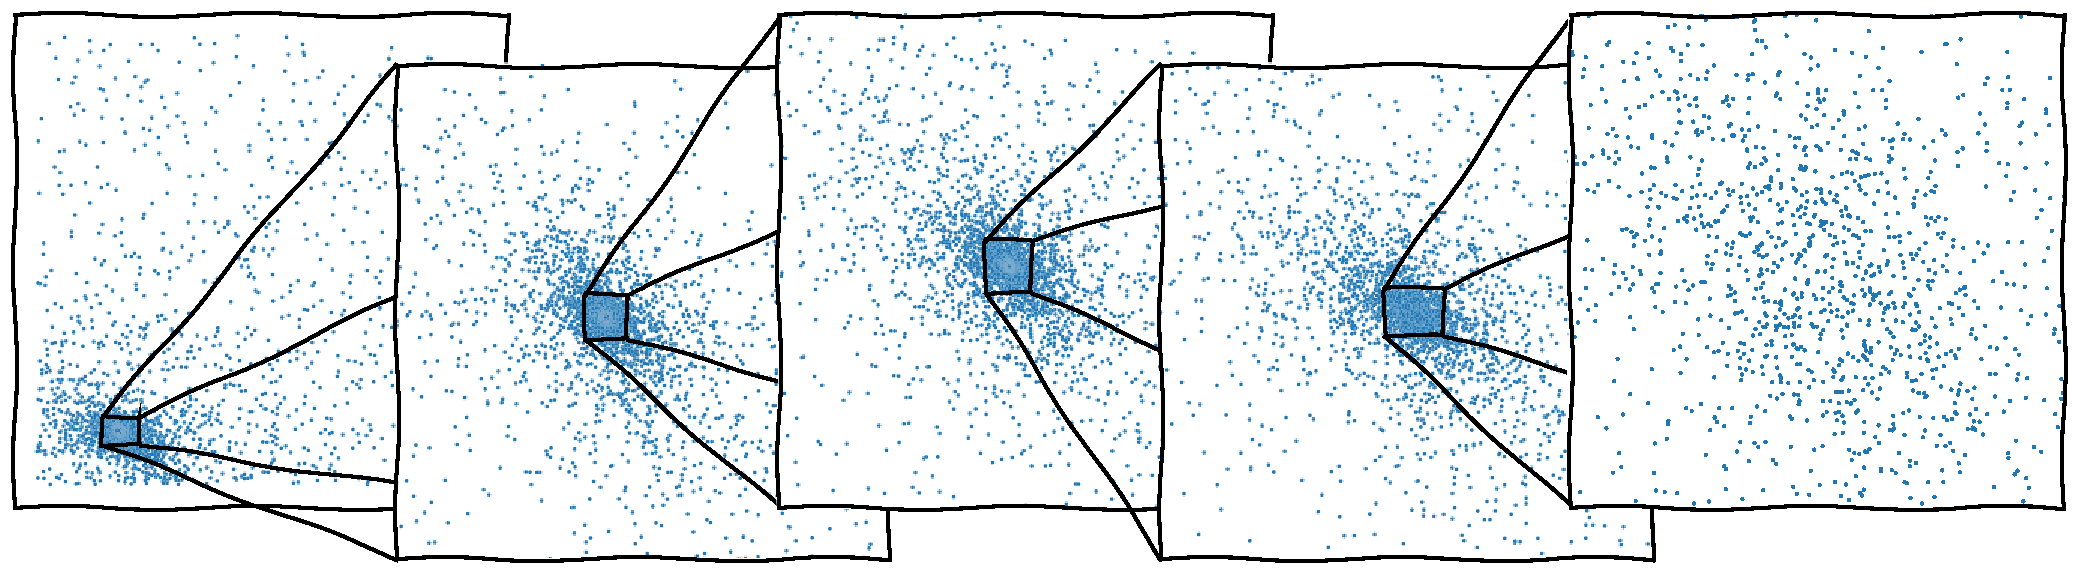
\includegraphics[width=\textwidth]{figures/dead_measure}
    \begin{columns}
        \column{0.69\textwidth}
        \begin{itemize}
            \item At the end, one is left with a set of discarded ``dead'' points.
            \item Dead points have a unique scale-invariant distribution $\propto\: \tfrac{dV}{V}$.
            \item Uniform over original region, exponentially concentrating on region of interest (until termination volume).
            \item Good for training emulators (HERA~\arxiv{2108.07282}).
        \end{itemize}
        \column{0.3\textwidth}
        \begin{block}{Applications}
        \begin{itemize}
            \item training emulators.
            \item gridding simulations
            \item beta flows
            \item ``dead measure'' 
        \end{itemize}
        \end{block}
    \end{columns}
\end{frame}

\begin{frame}
    \frametitle{Implementations of Nested Sampling \arxiv{2205.15570}(NatReview)}
    \begin{columns}[t]
        \column{0.3\textwidth}
        \texttt{MultiNest}~\arxiv{0809.3437}
        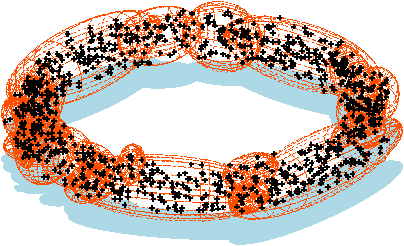
\includegraphics[width=\textwidth]{figures/multinest}
        \texttt{UltraNest}~\arxiv{2101.09604}
        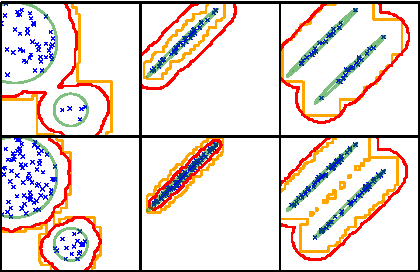
\includegraphics[width=\textwidth]{figures/radfriends}
        \texttt{nautilus}~\arxiv{2306.16923} 
        \column{0.4\textwidth}
        \texttt{PolyChord}~\arxiv{1506.00171}
        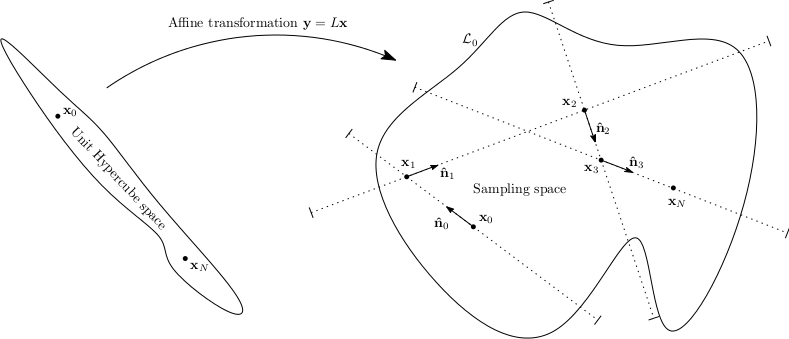
\includegraphics[width=\textwidth]{figures/polychord}
        \vfill
        \texttt{NeuralNest}~\arxiv{1903.10860}
        \begin{columns}
            \column{0.55\textwidth}
            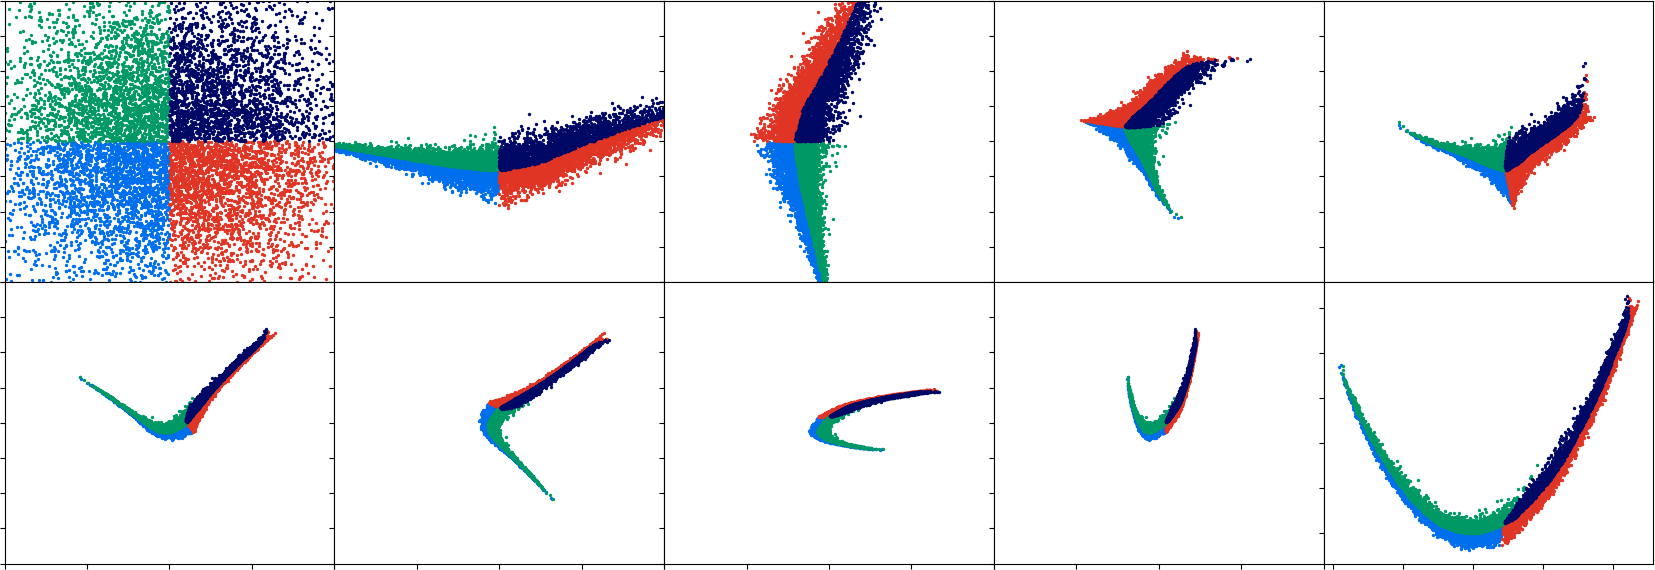
\includegraphics[width=\textwidth]{figures/rosenbrock_flow.png}
            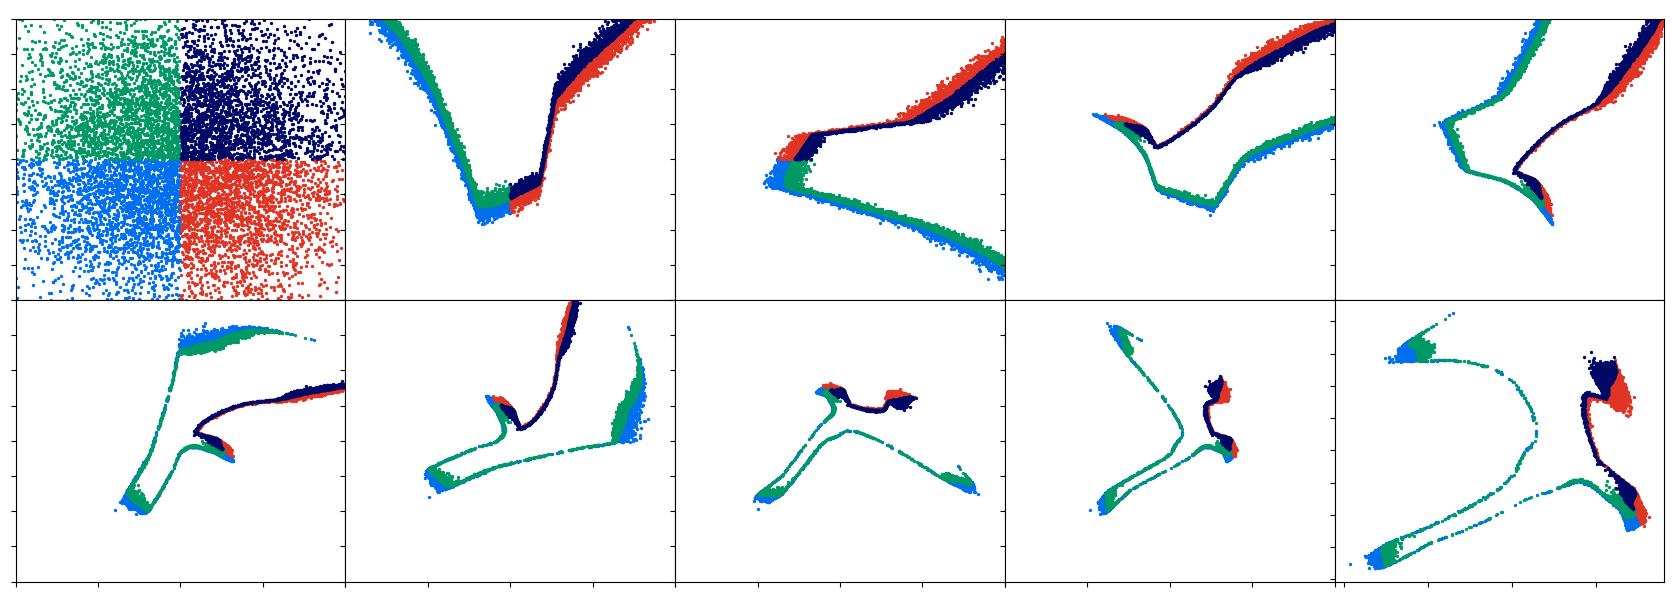
\includegraphics[width=\textwidth]{figures/himmelblau_flow.png}
            \column{0.45\textwidth}
            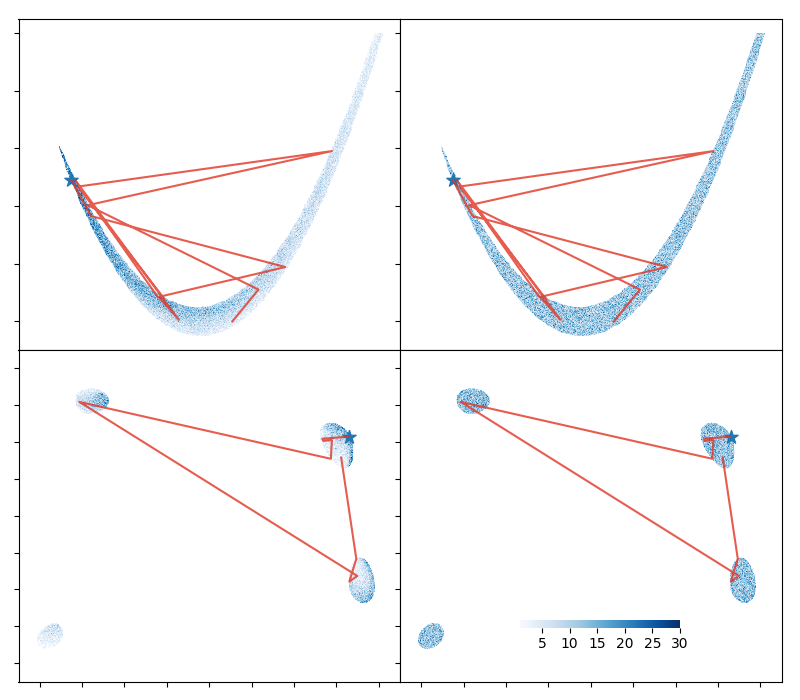
\includegraphics[width=\textwidth]{figures/chains.png}
        \end{columns}
        \texttt{nessai}~\arxiv{2102.11056} \texttt{nora}~\arxiv{2305.19267} \texttt{jaxnest}~\arxiv{2012.15286}
        \vfill
        \column{0.3\textwidth}
        \texttt{DNest}~\arxiv{1606.03757}
        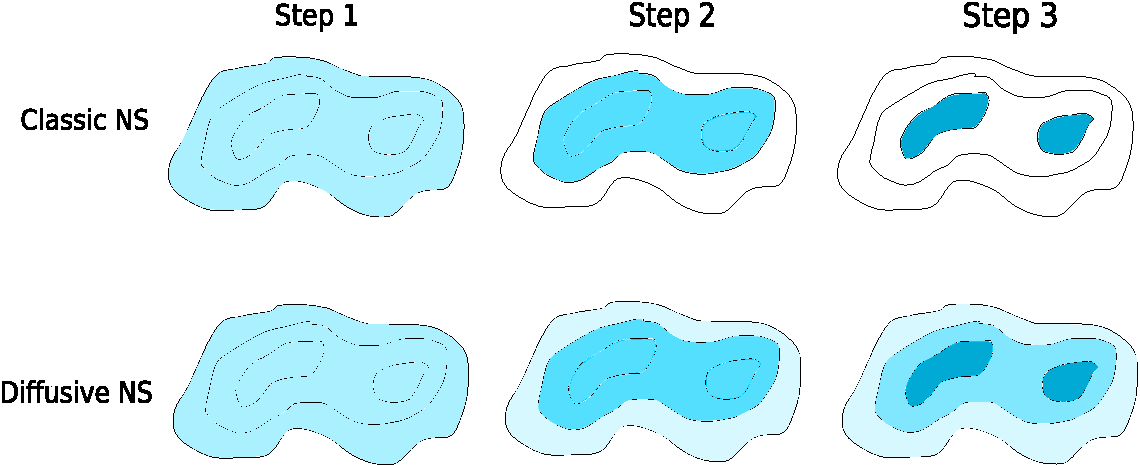
\includegraphics[width=\textwidth]{figures/dnest}
        \texttt{ProxNest}~\arxiv{2106.03646}
        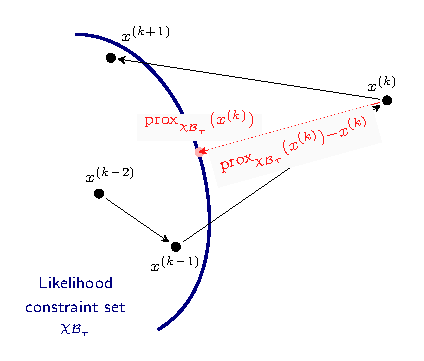
\includegraphics[width=\textwidth]{figures/proxnest_diagram}
        \texttt{dynesty}~\arxiv{1904.02180} 
        \vfill
    \end{columns}
\end{frame}

\begin{frame}
    \frametitle{Types of nested sampler}
    \begin{itemize}
        \item Broadly, most nested samplers can be split into how they create new live points.
        \item i.e. how they sample from the hard likelihood constraint $\{\theta\sim \pi : \mathcal{L}(\theta)>\mathcal{L}_* \}$.
    \end{itemize}
    \vspace{-10pt}
    \begin{columns}[t]
        \column{0.48\textwidth}
        \begin{block}{Rejection samplers}
            \begin{itemize}
                \item e.g. \texttt{MultiNest}, \texttt{UltraNest}.
\item Constructs bounding region and draws many invalid points until $\mathcal{L}(\theta)>\mathcal{L}_*$.
                \item Efficient in low dimensions, exponentially inefficient $\sim\mathcal{O}(e^{d/d_0})$ in high  $d>d_0\sim10$.
            \end{itemize}
        \end{block}
        \column{0.48\textwidth}
        \begin{block}{Chain-based samplers}
            \begin{itemize}
                \item e.g. \texttt{PolyChord}, \texttt{ProxNest}.
                \item Run Markov chain starting at a live point, generating many valid (correlated) points.
                \item Linear $\sim\mathcal{O}(d)$ penalty in decorrelating new live point from the original seed point.
            \end{itemize}
        \end{block}
    \end{columns}
    \vspace{5pt}
    \begin{itemize}
        \item Nested samplers usually come with:
            \begin{itemize}
                \item \emph{resolution} parameter $n_\mathrm{live}$ (which improve results as $\sim\mathcal{O}(n_\mathrm{live}^{-1/2})$.
                    \item set of \emph{reliability} parameters~\arxiv{2101.04525}, which don't improve results if set arbitrarily high, but introduce systematic errors if set too low.
                    \item e.g. \texttt{Multinest} efficiency \texttt{eff} or \texttt{PolyChord} chain length $n_\mathrm{repeats}$.
            \end{itemize}
    \end{itemize}
\end{frame}

\begin{frame}
    \frametitle{Applications of nested sampling}
    \framesubtitle{Cosmology}
    \student{adam_ormondroyd}{Adam Ormondroyd}{PhD}
    \begin{columns}
        \column{0.55\textwidth}
        \begin{itemize}
            \item Battle-tested in Bayesian cosmology on
                \begin{itemize}
                    \item Parameter estimation: multimodal alternative to MCMC samplers.
                    \item Model comparison: using integration to compute the Bayesian evidence
                    \item Tension quantification: using deep tail sampling and suspiciousness computations.
                \end{itemize}
            \item Plays a critical role in major cosmology pipelines: Planck, DES, KiDS, BAO, SNe.
            \item The default $\Lambda$CDM cosmology is well-tuned to have Gaussian-like posteriors for CMB data. 
            \item Less true for alternative cosmologies/models and orthogonal datasets, so nested sampling crucial.
        \end{itemize}
        \column{0.45\textwidth}
        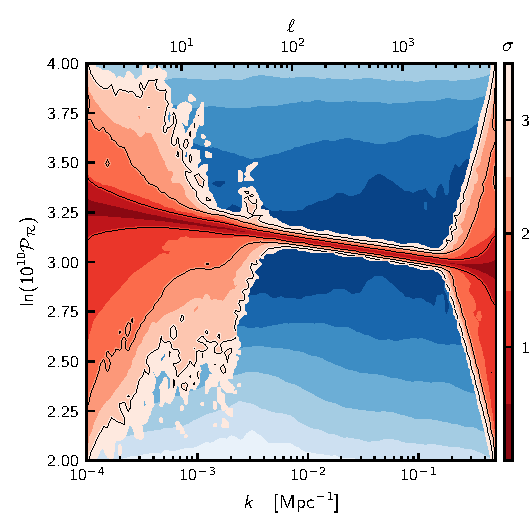
\includegraphics[width=0.49\textwidth]{figures/pps_both}
        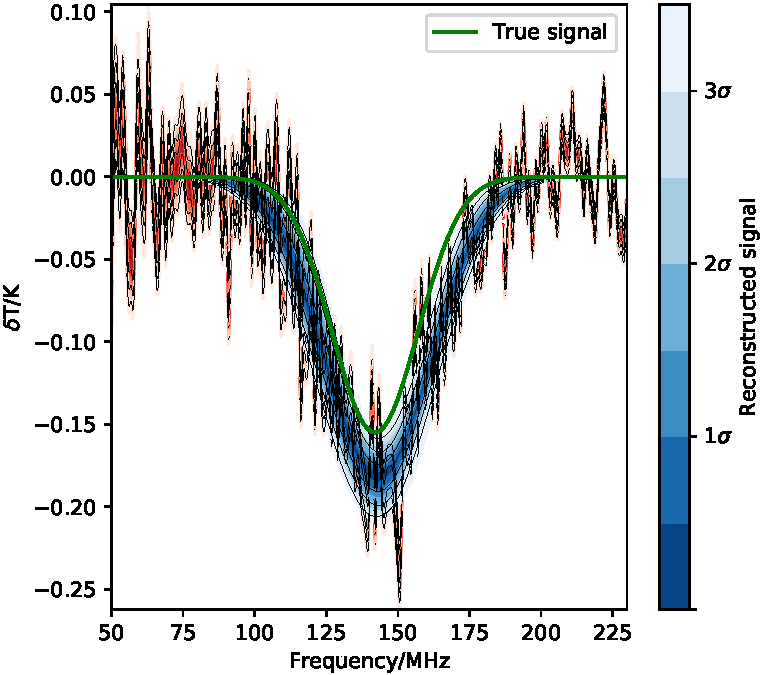
\includegraphics[width=0.49\textwidth]{figures/reach_fit-cropped.pdf}
        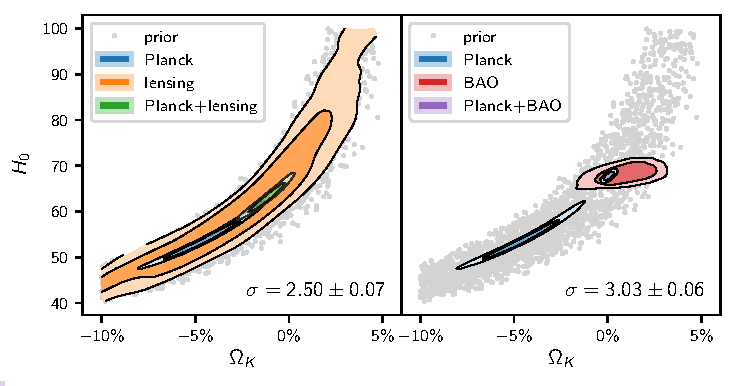
\includegraphics[width=\textwidth]{figures/omegak_H0_2.pdf}
    \end{columns}
\end{frame}

\begin{frame}
    \frametitle{Applications of nested sampling}
    \framesubtitle{Astrophysics}
\student{metha_prathaban}{Metha Prathaban}{PhD}
    \begin{columns}
        \column{0.6\textwidth}
        \begin{itemize}
            \item In exoplanets~\arxiv{1806.00518}
                \begin{itemize}
                    \item Parameter estimation: determining properties of planets.
                    \item Model comparison: how many planets? Stellar modelling~\arxiv{2007.07278}.
                    \item exoplanet problems regularly have posterior phase transitions \arxiv{2102.03387}
                \end{itemize}
            \item In gravitational waves
                \begin{itemize}
                    \item Parameter estimation: Binary merger properties
                    \item Model comparison: Modified theories of gravity, selecting phenomenological parameterisations~\arxiv{1803.10210}
                    \item Likelihood reweighting: fast slow properties
                \end{itemize}
        \end{itemize}
        \column{0.4\textwidth}
        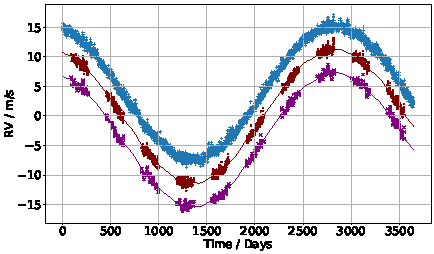
\includegraphics[width=\textwidth]{figures/rv_full.pdf}
        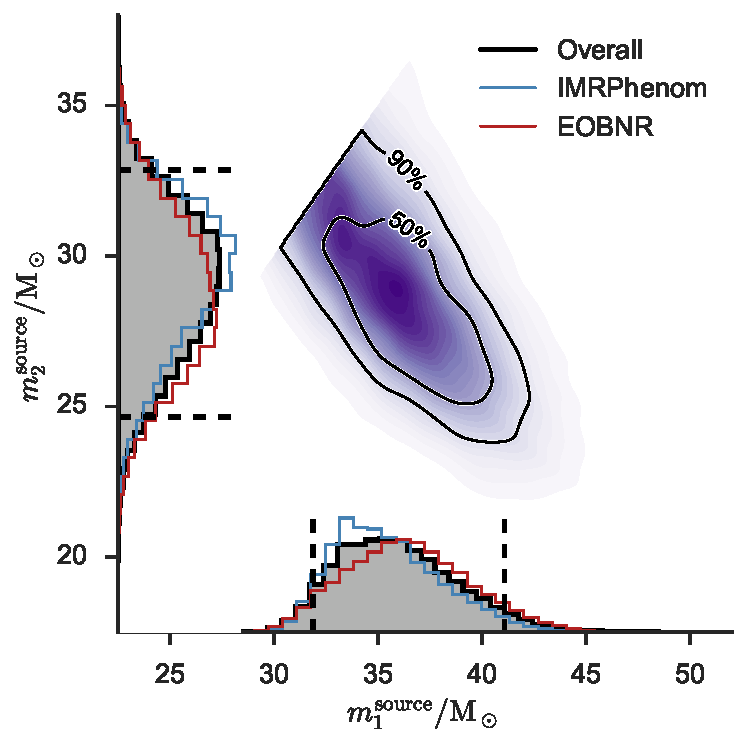
\includegraphics[width=0.49\textwidth]{figures/ligo_m1_m2.pdf}
        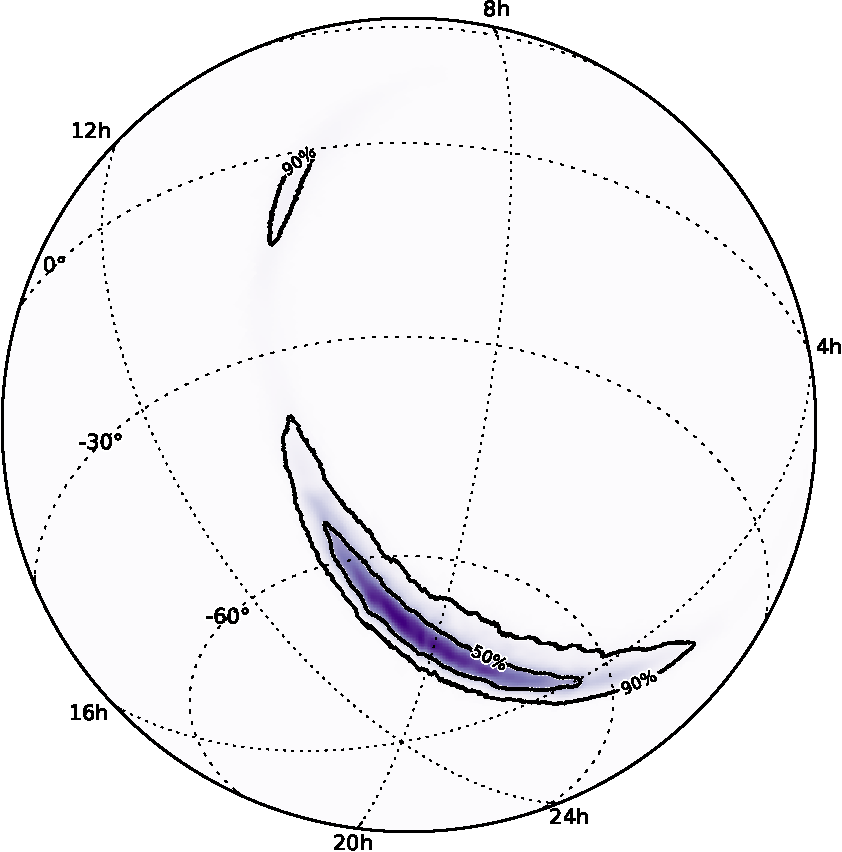
\includegraphics[width=0.49\textwidth]{figures/ligo_lambert-skymap.pdf}
    \end{columns}
\end{frame}

\begin{frame}
    \frametitle{Applications of nested sampling}
    \framesubtitle{Particle physics}
    \student{david_yallup}{David Yallup}{PDRA}
    \begin{columns}
        \column{0.56\textwidth}
        \begin{columns}
            \column{0.67\textwidth}
            \begin{itemize}
                \item Nested sampling for cross section computation/event generation
            \end{itemize}
            \column{0.3\textwidth}
            \[\sigma = \int_\Omega d\Phi |\mathcal{M}|^2.\]
        \end{columns}
        \begin{itemize}
            \item Nested sampling can explore the phase space $\Omega$ and compute integral blind with comparable efficiency to HAAG/RAMBO~\arxiv{2205.02030}.
            \item Bayesian sparse reconstruction~\arxiv{1809.04598} applied to bump hunting allows evidence-based detection of signals in phenomenological backgrounds~\arxiv{2211.10391}.
            \item Fine tuning quantification
            \item Fast estimation of small $p$-values \arxiv{2106.02056}(PRL), just make switch:\\ $X\leftrightarrow p$, $\mathcal{L}\leftrightarrow\lambda$, $\theta \leftrightarrow x$.
        \end{itemize}
        \column{0.17\textwidth}
        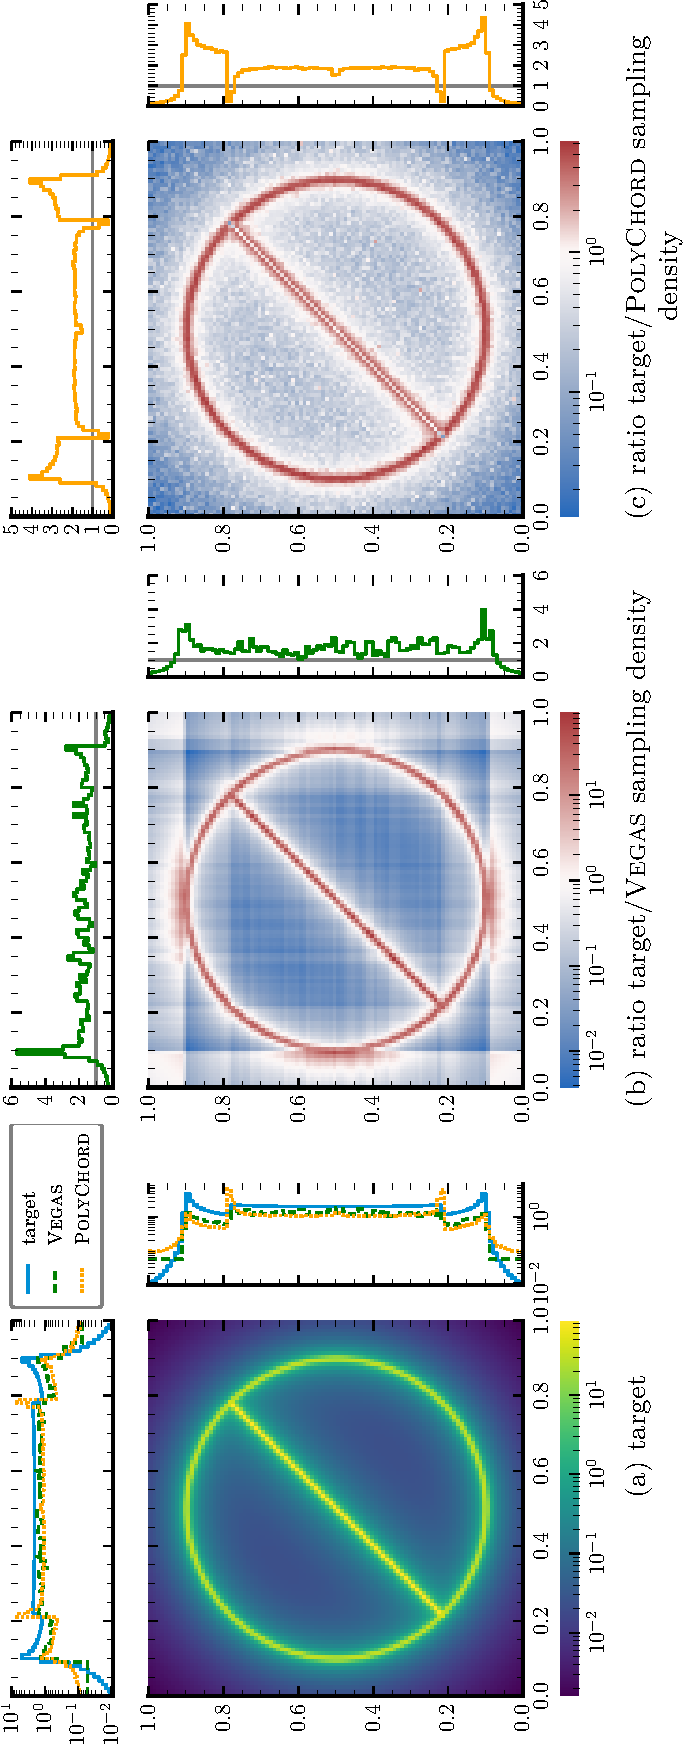
\includegraphics[width=\textwidth]{figures/phase_space_1-pdfjam-crop.pdf}
        \column{0.27\textwidth}
        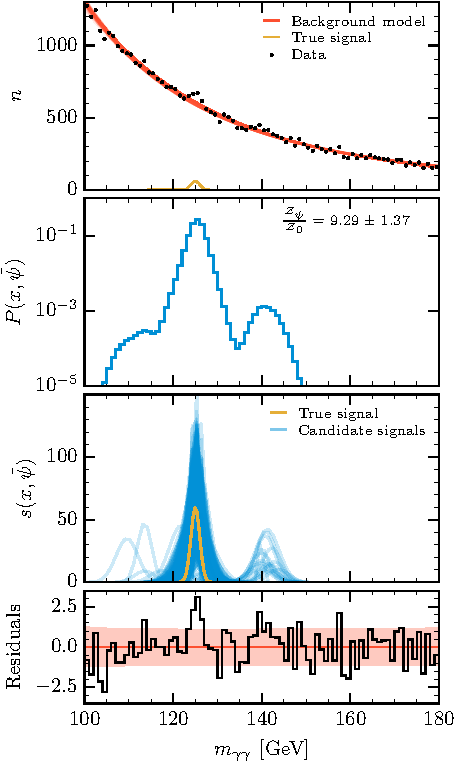
\includegraphics[width=\textwidth]{figures/psi_predict-crop.pdf}
    \end{columns}
\end{frame}

\begin{frame}
    \frametitle{Applications of nested sampling}
    \framesubtitle{Lattice field theory}
\student{david_yallup}{David Yallup}{PDRA}
    \begin{columns}
        \column{0.5\textwidth}
        \begin{itemize}
            \item Consider standard field theory Lagrangian:
                \[ Z(\beta) = \int D\phi e^{-\beta S(\phi)}, \quad S(\phi) = \int dx^\mu \mathcal{L}(\phi) \]
            \item Discretize onto spacetime grid.
            \item Compute partition function
            \item NS unique traits:
                \begin{itemize}
                    \item Get full partition function for free
                    \item allows for critical tuning
                    \item avoids critical slowing down
                \end{itemize}
            \item Applications in lattice gravity, QCD, condensed matter physics
        \end{itemize}
        \column{0.5\textwidth}
        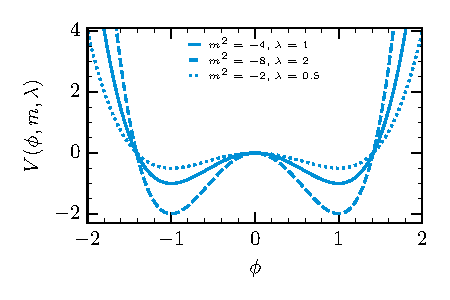
\includegraphics[width=0.49\textwidth]{figures/potential_shape}
        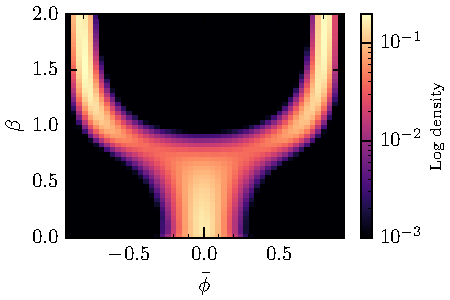
\includegraphics[width=0.49\textwidth]{figures/2d_phase}
        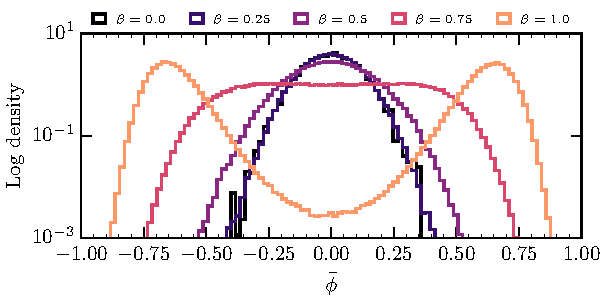
\includegraphics[width=\textwidth]{figures/lattice_field_theory.pdf}
    \end{columns}
\end{frame}

\begin{frame}
    \frametitle{Applications of nested sampling}
    \framesubtitle{Machine learning}
\student{kamran_javid}{Kamran Javid}{PDRA}
    \begin{columns}
        \column{0.62\textwidth}
        \begin{itemize}
            \item Machine learning requires:
                \begin{itemize}
                    \item Training to find weights
                    \item Choice of architecture/topology/hyperparameters
                \end{itemize}
            \item Bayesian NNs treat training as a model fitting problem
            \item Compute posterior of weights (parameter estimation), rather than optimisation (gradient descent)
            \item Use evidence to determine best architecture (model comparison), correlates with out-of-sample performance! 
            \item Solving the full ``shallow learning'' problem without compromise \arxiv{2004.12211}\arxiv{2211.10391}. 
                \begin{itemize}
                    \item Promising work ongoing to extend this to transfer learning and deep nets.
                \end{itemize}
            \item More generally, dead points are optimally spaced  for training traditional ML approaches e.g. \arxiv{2309.05697}
        \end{itemize}
        \column{0.38\textwidth}
        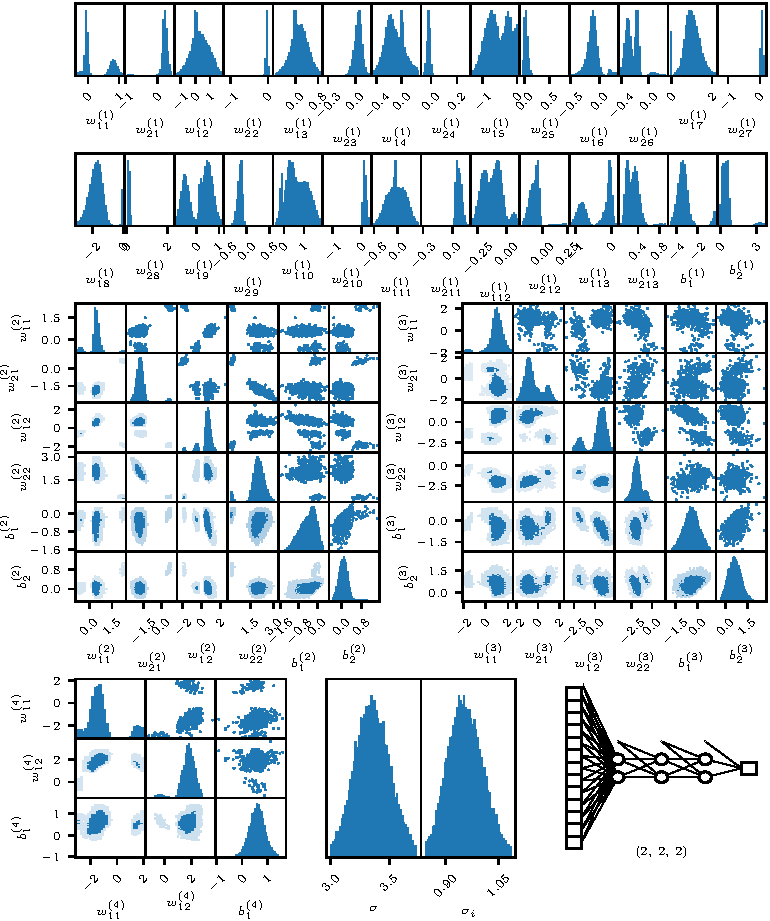
\includegraphics[width=\textwidth]{figures/nn_posterior-cropped.pdf}
    \end{columns}
\end{frame}

\begin{frame}
    \frametitle{Applications of nested sampling}
    \framesubtitle{And beyond\ldots}
    \only<1-4>{
        \student{catherine-watkinson-polychord}{Catherine Watkinson}{Senior Data Scientist}
    }
    \only<5->{
        \student{thomas-macaloone-polychord}{Thomas Mcaloone}{PhD $\to$ Data Scientist}
    }
    \begin{columns}
        \column{0.6\textwidth}
        \begin{itemize}
            \item Techniques have been spun-out (PolyChord Ltd) to:
            \item Protein folding
                \begin{itemize}
                    \item Navigating free energy surface.
                    \item Computing misfolds.
                    \item Thermal motion.
                \end{itemize}
            \item Nuclear fusion reactor optimisation
                \begin{itemize}
                    \item multi-objective.
                    \item uncertainty propagation.
                \end{itemize}
            \item Telecoms \& DSTL research (MIDAS)
                \begin{itemize}
                    \item Optimising placement of transmitters/sensors.
                    \item Maximum information data acquisition strategies.
                \end{itemize}
        \end{itemize}
        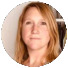
\includegraphics[width=0.08\textwidth]{people/catherine-watkinson-polychord.jpg}%
        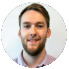
\includegraphics[width=0.08\textwidth]{people/thomas-macaloone-polychord.jpg}%
        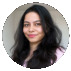
\includegraphics[width=0.08\textwidth]{people/parul-janagal-polychord.jpg}%
        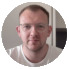
\includegraphics[width=0.08\textwidth]{people/angus-peters-polychord.jpg}%
        
\includegraphics[width=0.08\textwidth]{people/tamas-stenzel-polychord.jpg}%
        
\includegraphics[width=0.08\textwidth]{people/david-yallup-polychord.jpg}%
        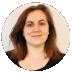
\includegraphics[width=0.08\textwidth]{people/rebecca-handley-polychord.jpg}%
        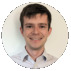
\includegraphics[width=0.08\textwidth]{people/adam-ormondroyd-polychord.jpg}%
        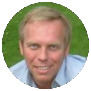
\includegraphics[width=0.08\textwidth]{people/mike-hobson-polychord.jpg}%
        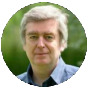
\includegraphics[width=0.08\textwidth]{people/anthony-lasenby-polychord.jpg}%
        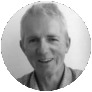
\includegraphics[width=0.08\textwidth]{people/mike-handley-polychord.jpg}%
        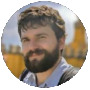
\includegraphics[width=0.08\textwidth]{people/will-handley-polychord.jpg}%
        \column{0.4\textwidth}
        \includegraphics<1|handout:0>[width=\textwidth]{figures/protein_1.png}%
        \includegraphics<2          >[width=\textwidth]{figures/protein_2.png}%
        \includegraphics<3|handout:0>[width=\textwidth]{figures/protein_3.png}%
        \includegraphics<4|handout:0>[width=\textwidth]{figures/lcoe.png}%
        \includegraphics<5|handout:0>[width=\textwidth]{figures/DKL_contour-cropped-crop.pdf}%
        \includegraphics<6|handout:0>[width=\textwidth]{figures/mean_DKL_optimise-3-crop.pdf}%
        \includegraphics<7|handout:0>[width=\textwidth]{figures/mean_DKL_optimise-4-crop.pdf}%
        \includegraphics<8|handout:0>[width=\textwidth]{figures/mean_DKL_optimise-5-crop.pdf}%
    \end{columns}
\end{frame}

\begin{frame}
    \frametitle{REACH: Global 21cm cosmology {\small \arxiv{2210.07409}(NatAstro)}}
    \student{ian_roque}{Ian Roque}{PhD}
    \vspace{10pt}
    \begin{columns}
        \column{0.65\textwidth}
        \vspace{-10pt}
        \begin{itemize}
            \item Imaging the universal dark ages using CMB backlight.
            \item $21\text{cm}$ hyperfine line emission from neutral hydrogen.
            \item Global experiments measure monopole across frequency.
            \item Challenge: science hidden in foregrounds $\sim 10^4\times$signal.
            \item Lead data analysis team (REACH first light in January)
            \item Nested sampling woven in from the ground up (calibrator, beam modelling, signal fitting, likelihood selection).
            \item All treated as parameterised model comparison problems.
        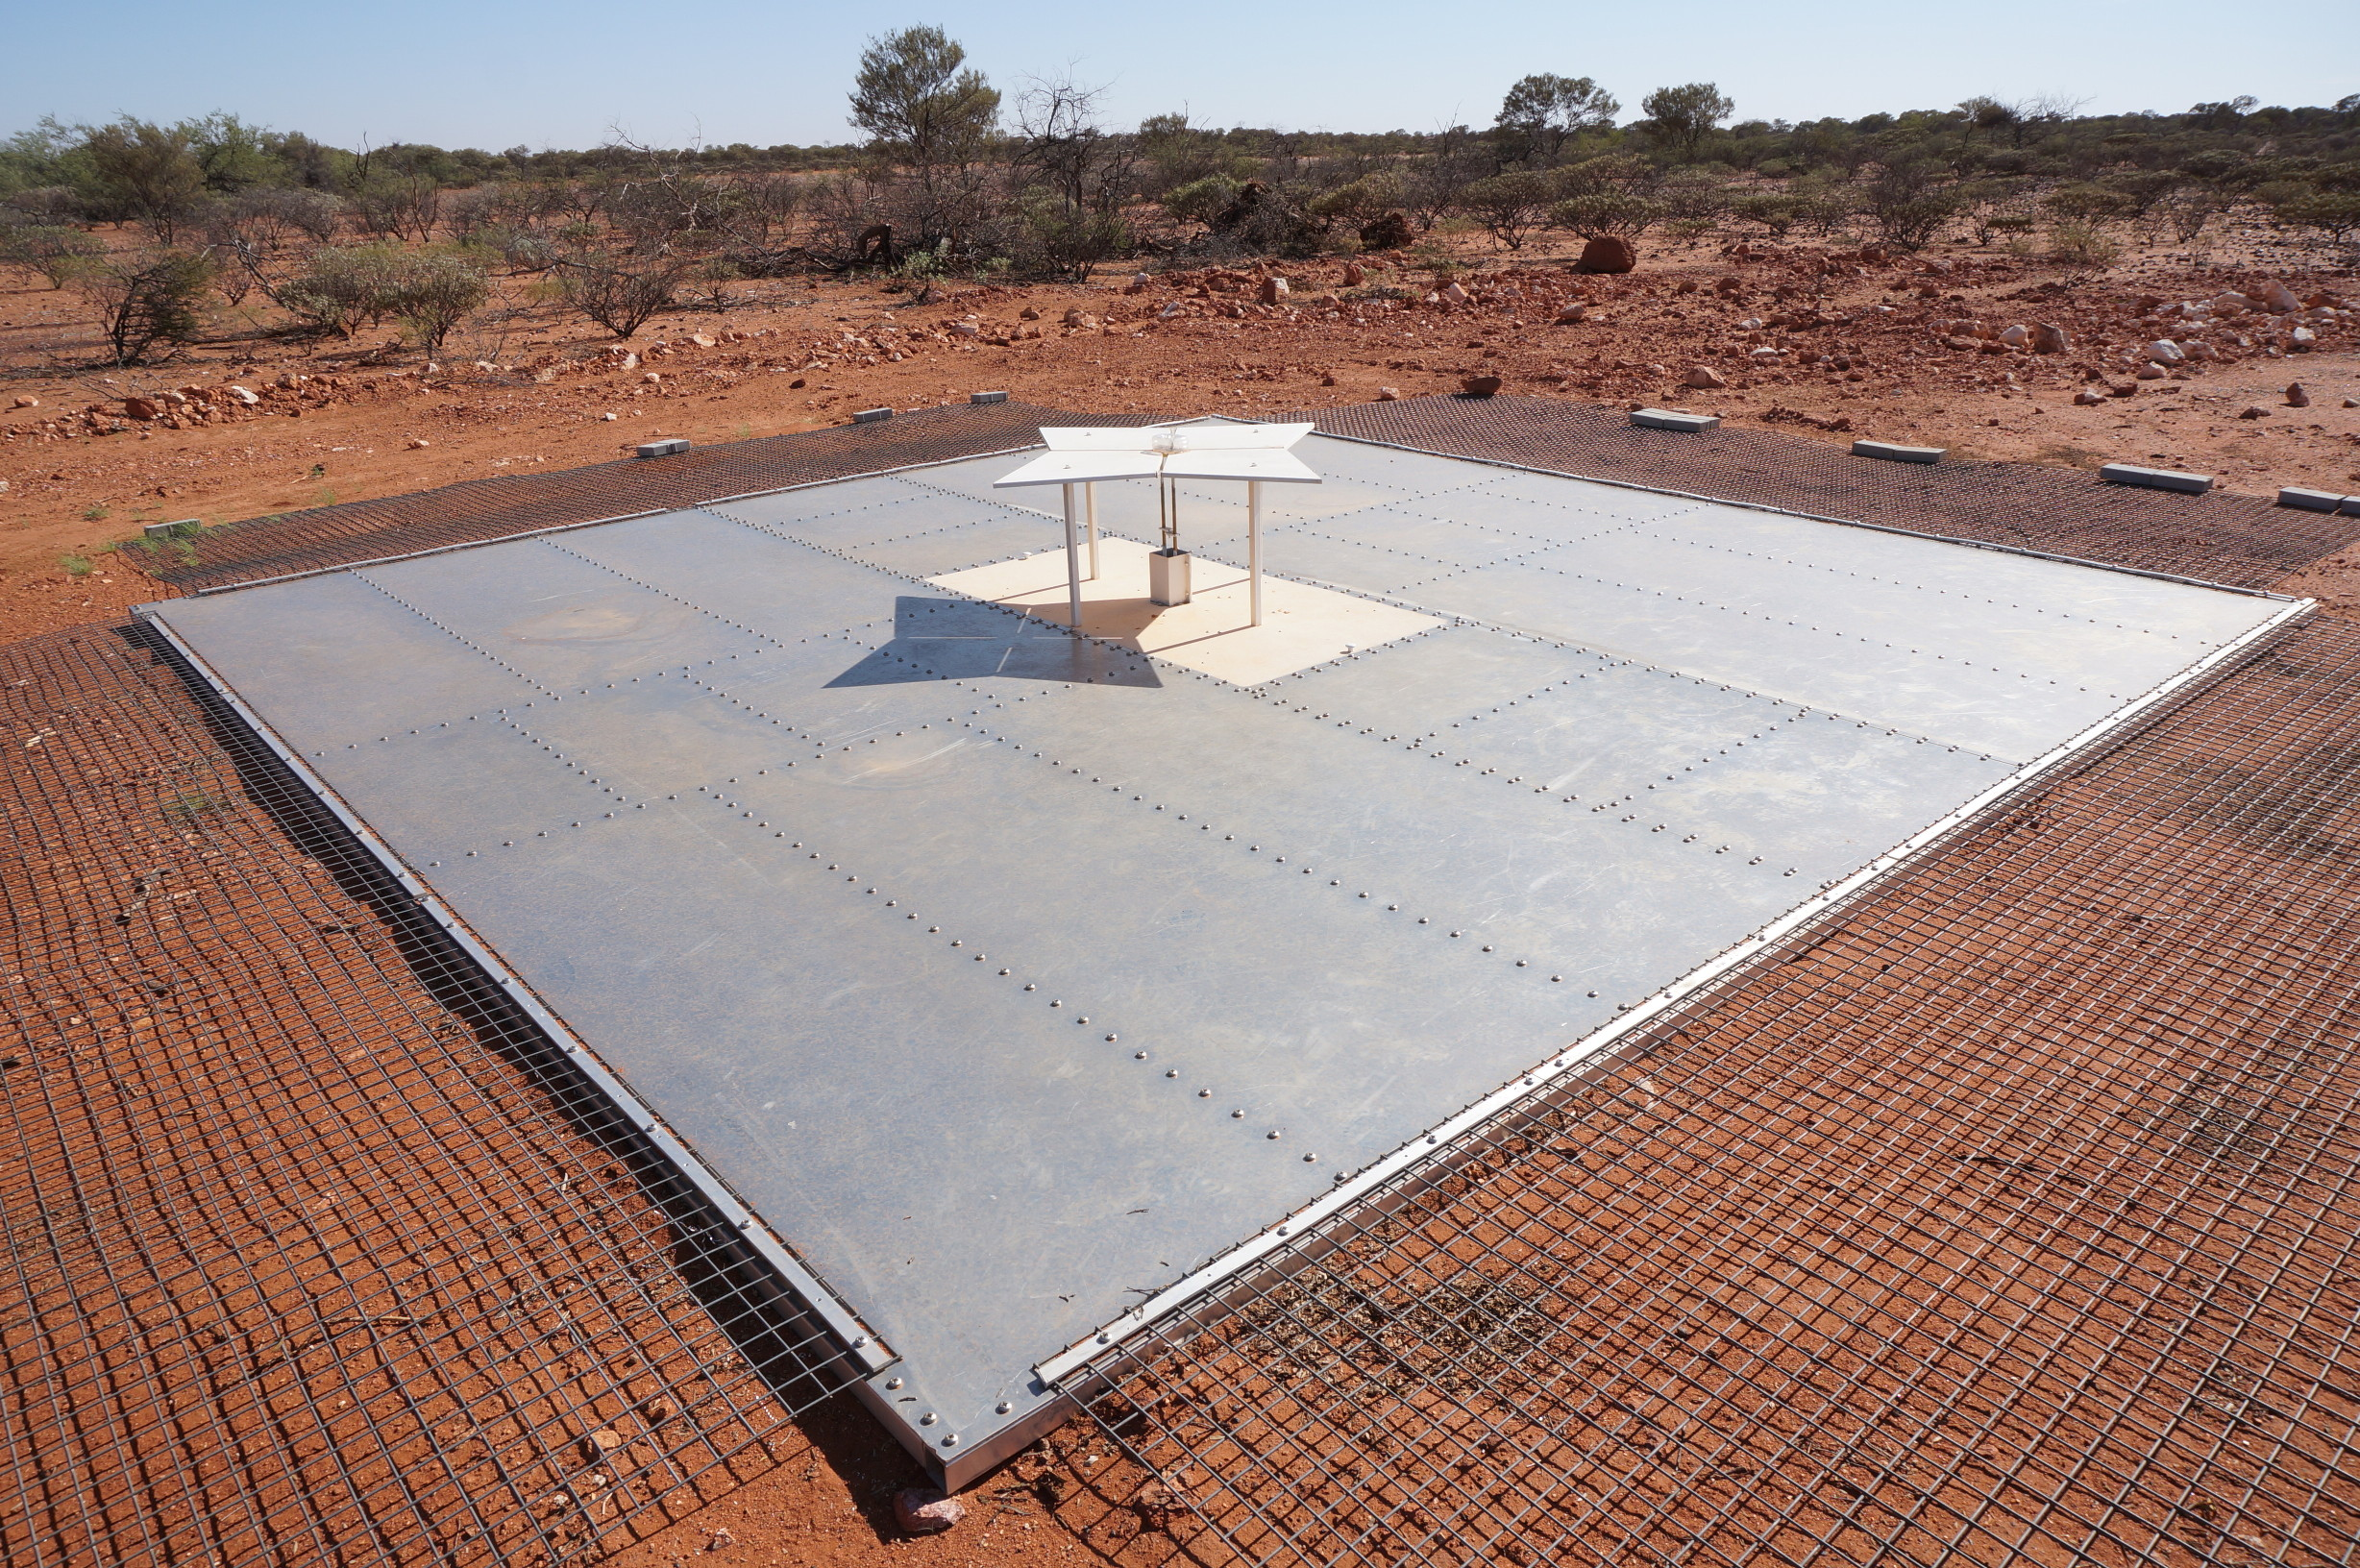
\includegraphics[height=0.3\textwidth]{figures/EDGES_antenna}
        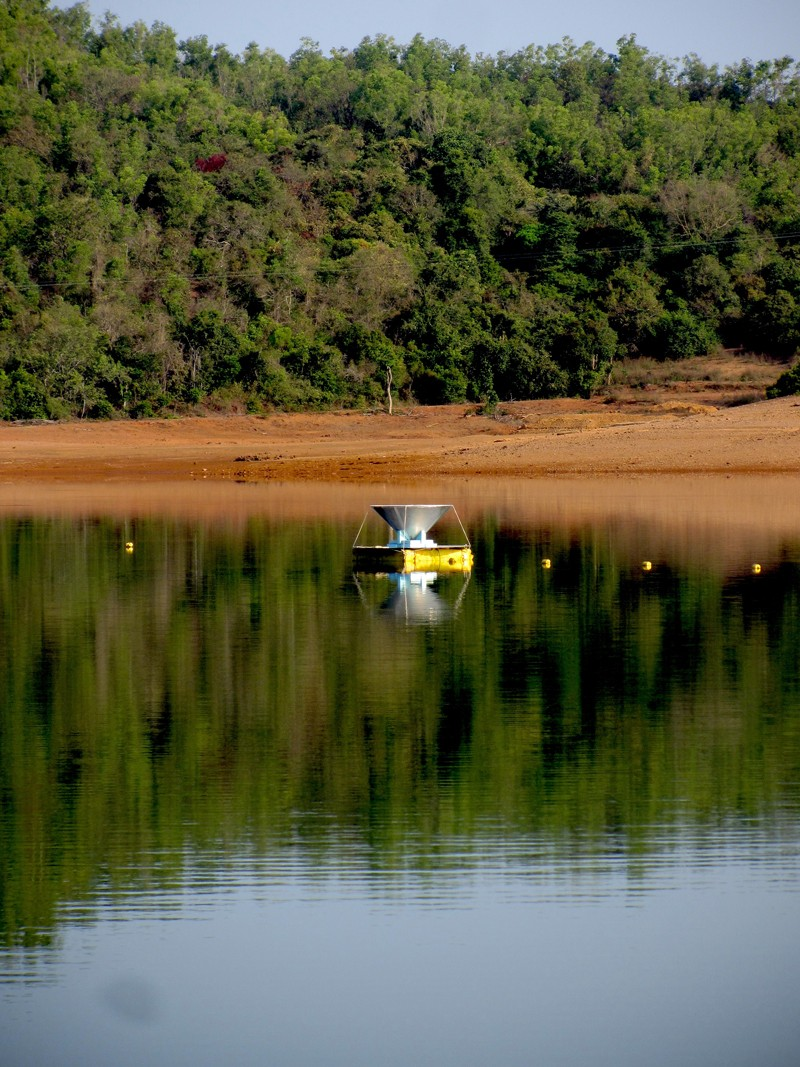
\includegraphics[height=0.3\textwidth]{figures/SARAS}
        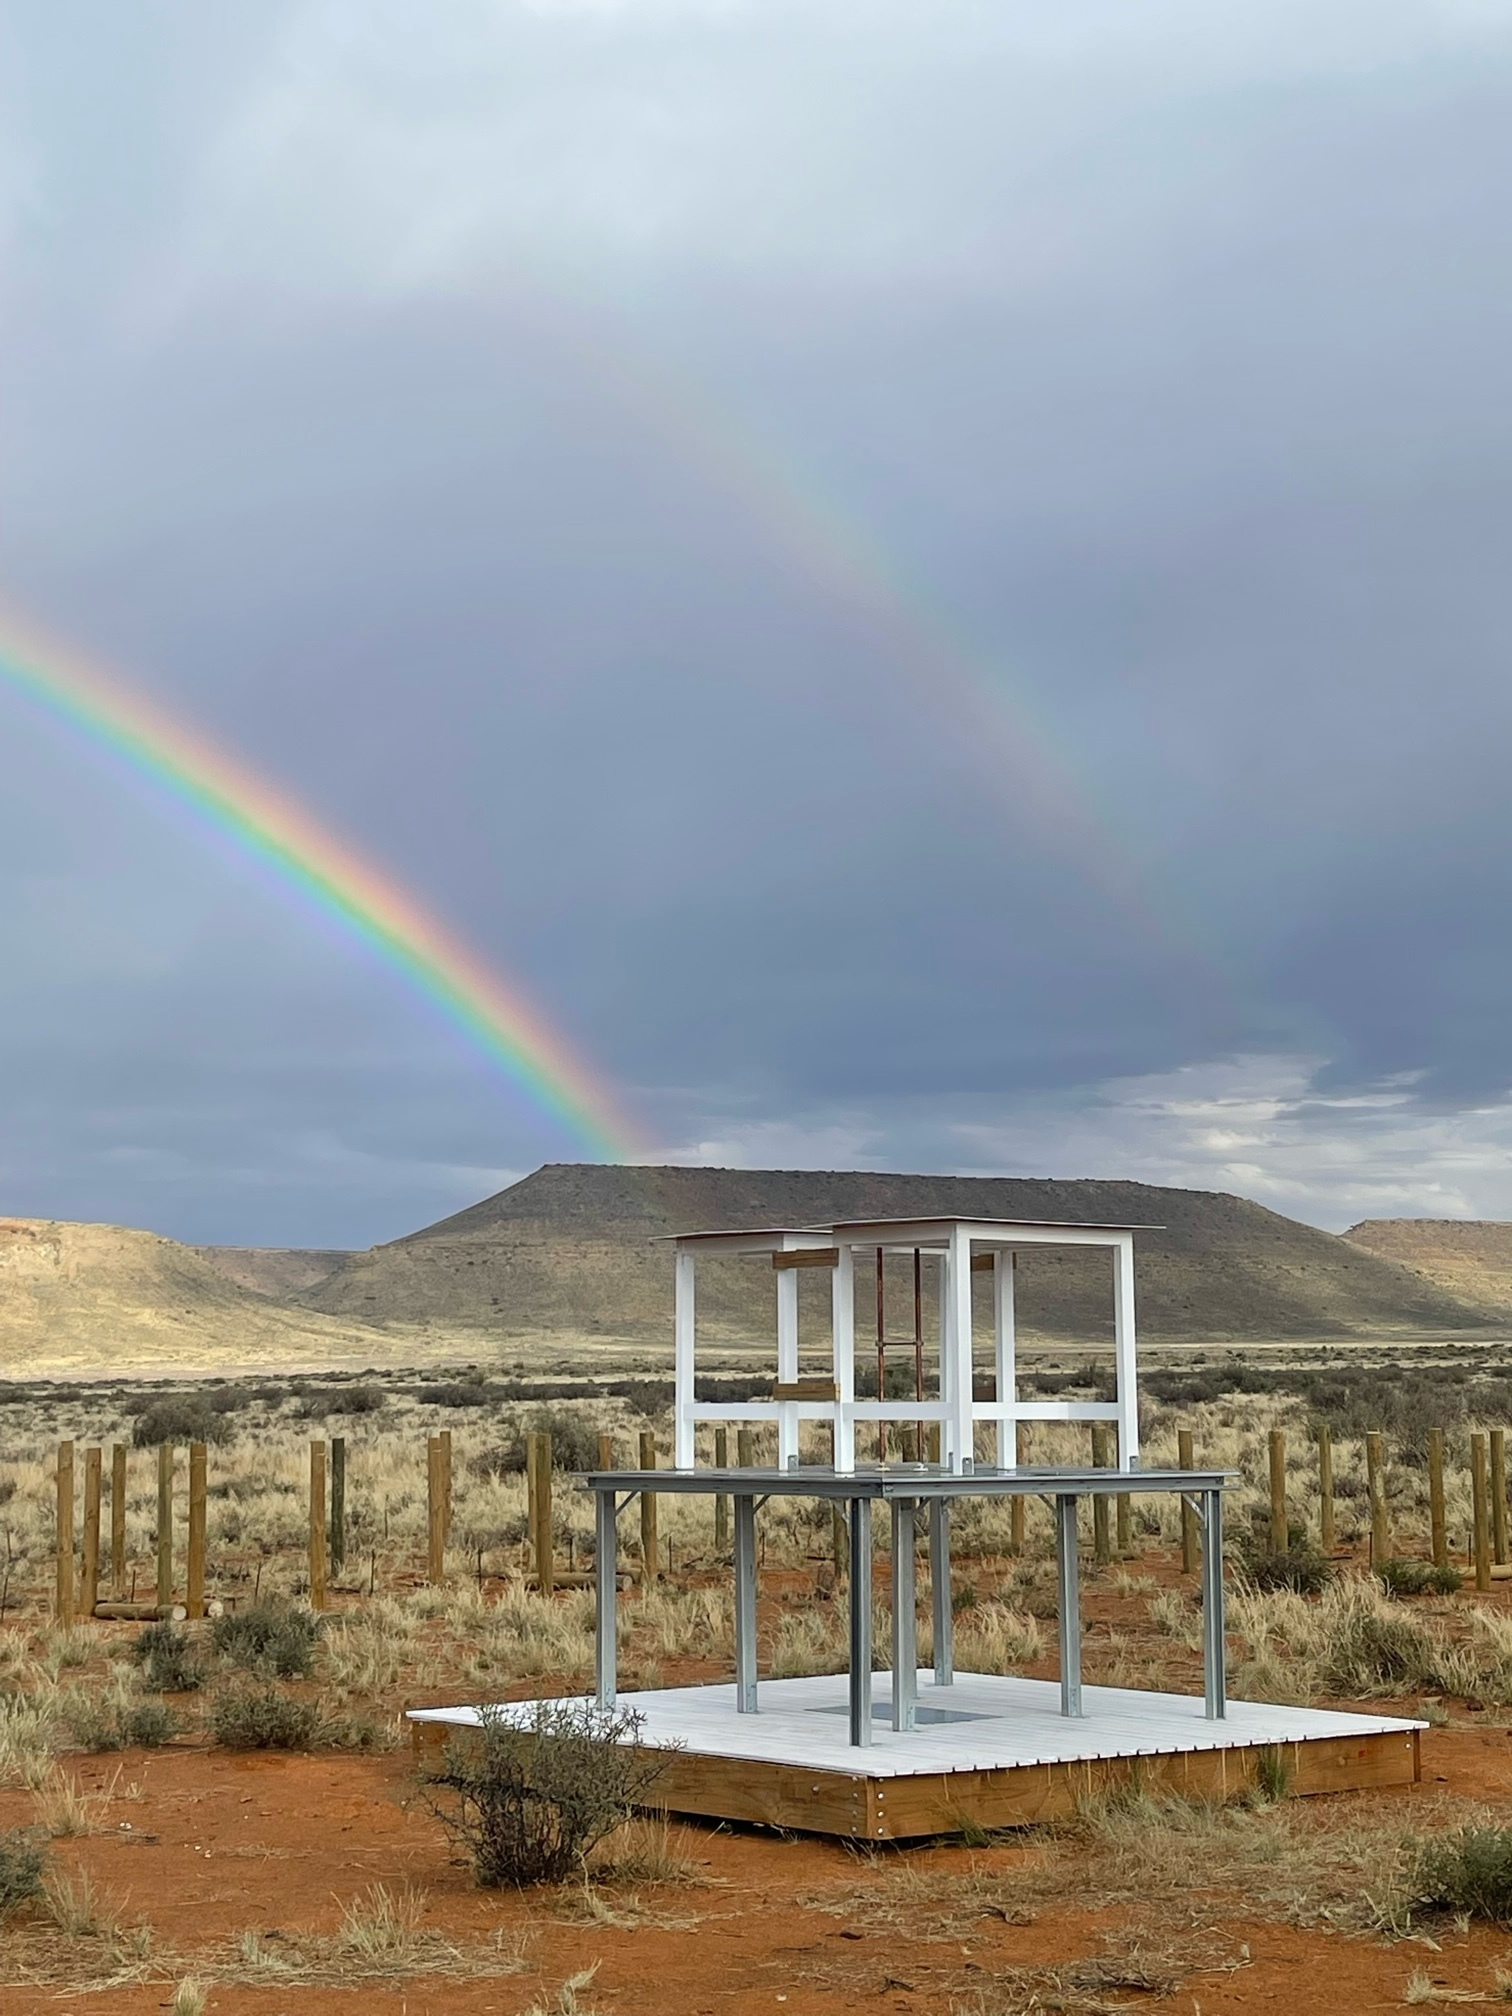
\includegraphics[height=0.3\textwidth]{figures/REACH_2.jpg}
        \end{itemize}
        \column{0.35\textwidth}
        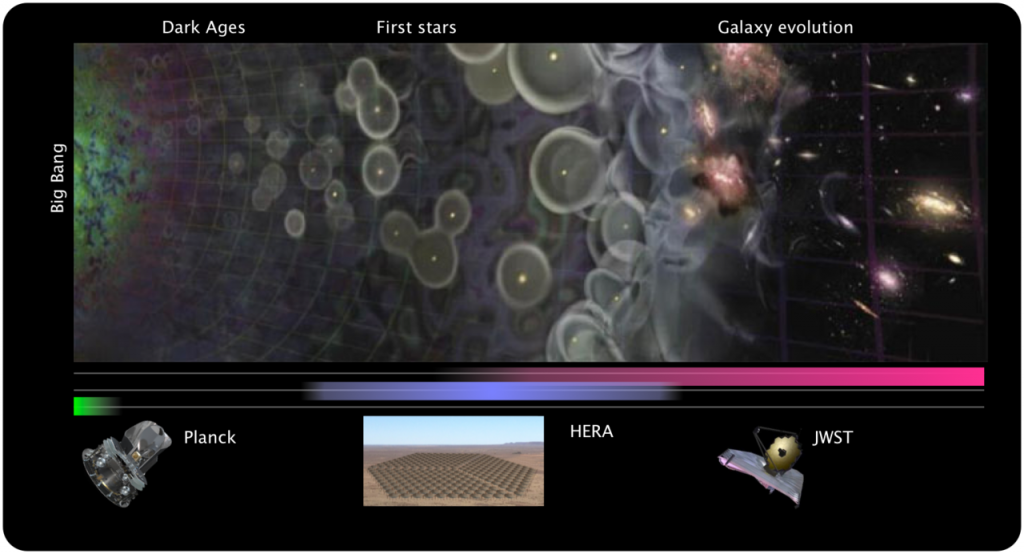
\includegraphics[width=\textwidth]{figures/21cm_1.png}
        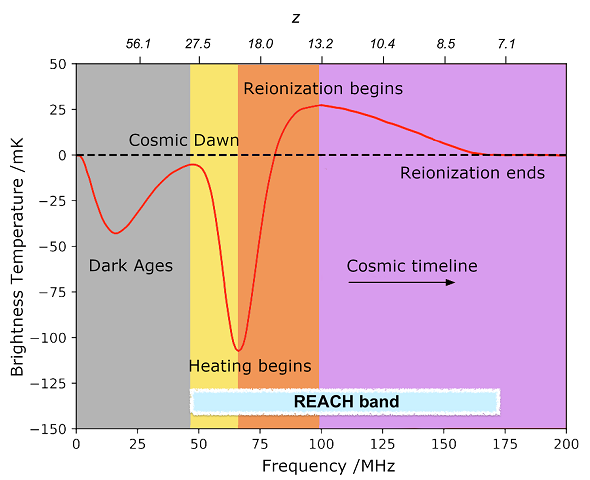
\includegraphics[width=\textwidth]{figures/21cm.png}
    \end{columns}
\end{frame}

\begin{frame}
    \frametitle{GAMBIT}
    \framesubtitle{Interdisciplinary case studies}
    \begin{columns}
        \column{0.5\textwidth}
        \begin{itemize}
            \item GAMBIT is an interdisciplinary community and software framework.
            \item Like \texttt{CosmoMC}/\texttt{Cobaya}/\texttt{Bilby}, an organiser of data, likelihoods \& theory, including:
                \begin{itemize}
                    \item Collider data (e.g. LHC)
                    \item Direct detections (e.g. XENON1T)
                    \item Cosmology (\texttt{MontePython})
                    \item Astrophysics (e.g. Bullet Cluster, Supernovae)
                    \item Pulsar timing
                    \item \ldots \& much more
                \end{itemize}
            \item \texttt{GravBit} and \texttt{LowEnergyBit} arising from GAMBIT@KICC workshop
        \end{itemize}
        \column{0.5\textwidth}
        
\includegraphics[height=0.423\textwidth]{people/gambit.png}
        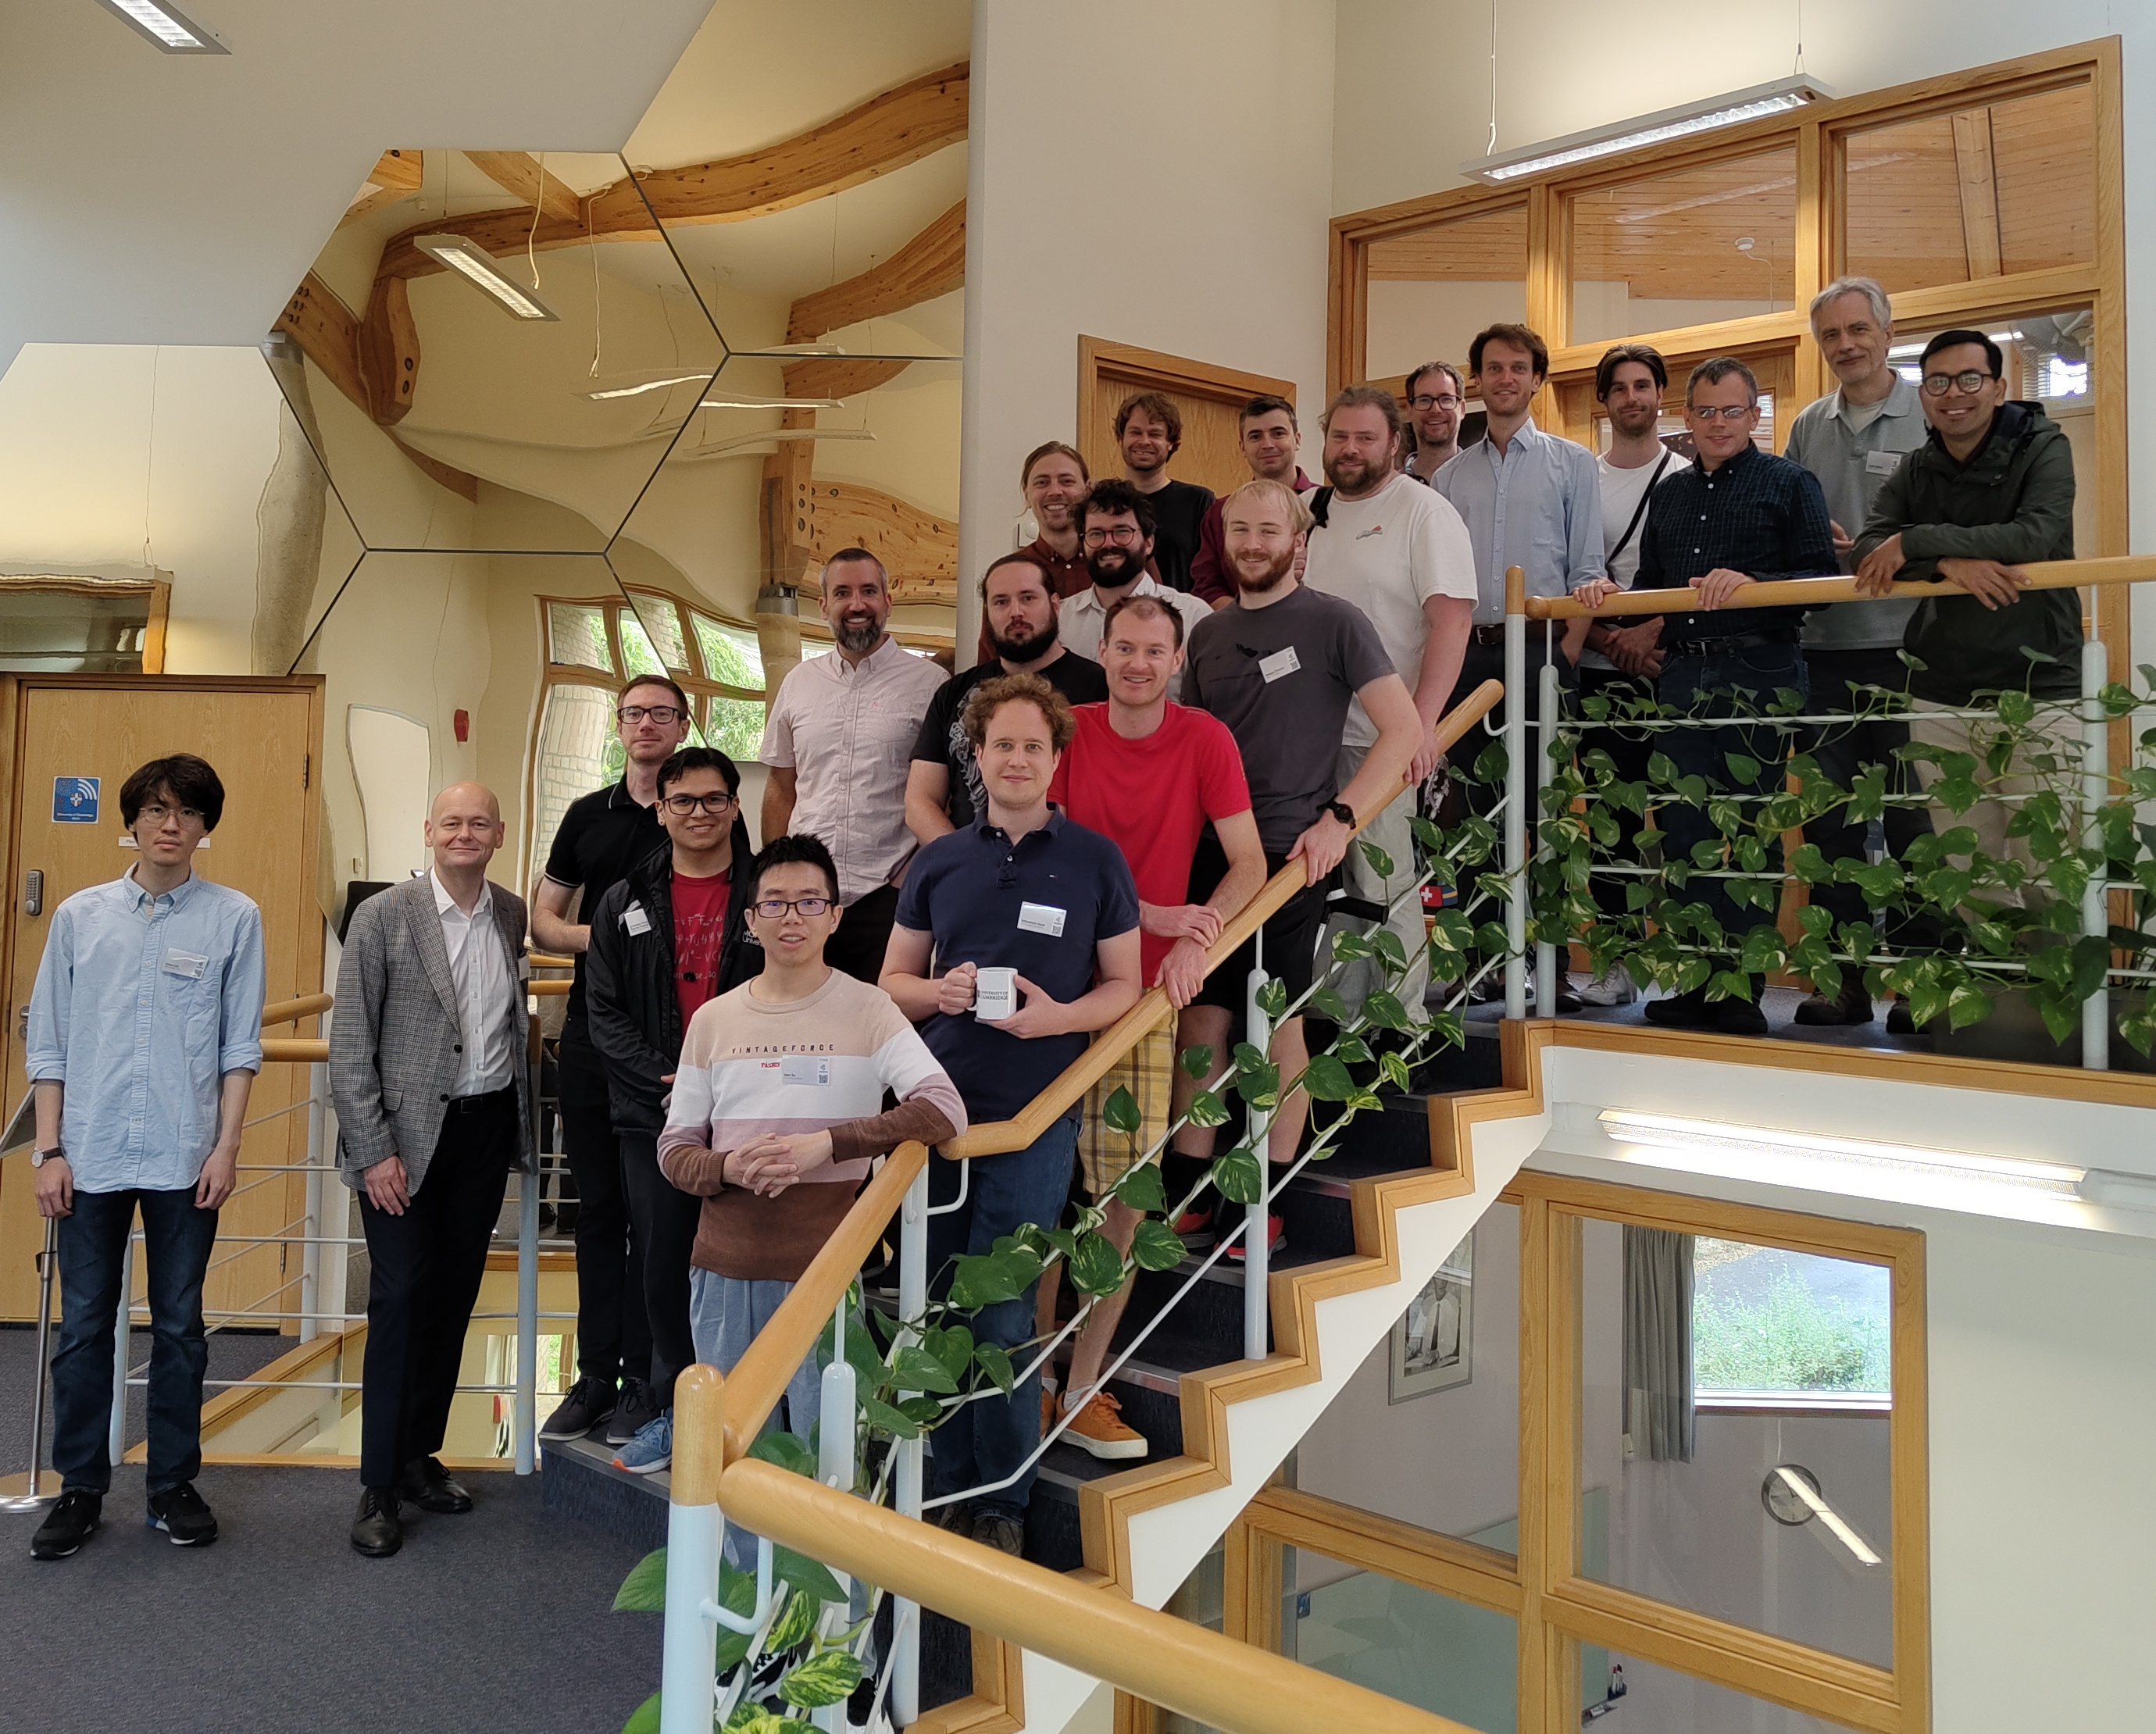
\includegraphics[height=0.423\textwidth]{figures/gambit_kicc.jpg}
        \includegraphics[width=\textwidth]{figures/gambit_meetingbanner.jpg}
    \end{columns}
\end{frame}

\begin{frame}
    \frametitle{GAMBIT: sub-GeV Dark matter constraints}
    \framesubtitle{Interdisciplinary case studies}
    \student{gambit}{Felix Kahlhoefer et al}{GAMBIT cosmo/DM working group}
    \begin{columns}
        \column{0.56\textwidth}
        \begin{itemize}
            \item Physical model of sub-GeV thermal dark matter with a dark photon mediator~$A$:
        \end{itemize}
        \vspace{-10pt}
        \begin{align*}
            \small
            \mathcal{L}_\text{int} =& -\frac{1}{2} m_{A'}^2 A'^\mu A'_\mu - \frac{1}{4} A'^{\mu\nu}A'_{\mu\nu} -\kappa e A'^\mu \sum_{f} q_f \overline{f} \gamma_\mu f \,,
            \normalsize
        \end{align*}
        \vspace{-15pt}
        \begin{itemize}
            \item Constrain using cosmological, astrophysical, accelerator \& direct detection data.
            \item Bayesian Model comparison of Fermion~$\psi$ vs scalar~$\Phi$ models (scalar preferred).
        \end{itemize}
        \vspace{-10pt}
        \begin{align*}
            \small
            \mathcal{L}_\psi  =& \bar{\psi}(i \slashed{\partial} - m_\text{DM}) \psi + g_\text{DM} A'^\mu \bar{\psi} \gamma_\mu \psi \,,\\
            \mathcal{L}_\Phi  =& |\partial_\mu \Phi|^2 - m_\text{DM}^2 |\Phi|^2 - g_\text{DM}^2 A'_\mu A'^\mu |\Phi|^2 \\ &+ i g_\text{DM} A'^\mu \left[\Phi^\ast (\partial_\mu \Phi) - (\partial_\mu \Phi^\ast) \Phi\right]\,,
            \normalsize
        \end{align*}
        \column{0.44\textwidth}
        \vspace{10pt}
        \includegraphics[width=\textwidth]{figures/Bayes_SubGeVDM_fermion_RDprior_allDM_asym_observables.pdf}
    \end{columns}
\end{frame}

\begin{frame}
    \frametitle{SBI: Simulation-based inference}
    \begin{columns}
        \column{0.5\textwidth}
        \begin{itemize}
            \item What do you do if you don't know \C[2]{$\mathcal{L}(D|\theta)$}?
            \item If you have a simulator/forward model $\theta \rightarrow D$
                defines an \C[2]{\emph{implicit} likelihood~$\mathcal{L}$}.
            \item Simulator generates samples from $\C[2]{\mathcal{L}(\cdot|\theta)}$.
            \item With a prior $\C[1]{\pi}(\theta)$ can generate samples from \C[4]{joint distribution}~$\C[4]{\mathcal{J}(\theta,D)}=\C[2]{\mathcal{L}(D|\theta)}\C[1]{\pi(\theta)}$\\\hfill \emph{the ``probability of everything''}.
            \item Task of SBI is take joint~$\C[4]{\mathcal{J}}$ samples and learn \C[0]{posterior $\mathcal{P}(\theta|D)$} and \C[3]{evidence $\mathcal{Z}(D)$} \\\hfill and possibly \C[2]{likelihood $\mathcal{L}(D|\theta)$}.
            \item Present state of the art achieves this using \emph{machine learning} (neural networks).
                \begin{itemize}
                    \item My group's research tries to removes machine learning \tthref{github.com/handley-lab/lsbi}.
                \end{itemize}
        \end{itemize}
        \column{0.5\textwidth}
        \includegraphics<1>[page=1, width=\textwidth]{figures/sbi_parameter_estimation.pdf}%
        \includegraphics<2>[page=2, width=\textwidth]{figures/sbi_parameter_estimation.pdf}%
        \includegraphics<3>[page=3, width=\textwidth]{figures/sbi_parameter_estimation.pdf}%
        \includegraphics<4>[page=4, width=\textwidth]{figures/sbi_parameter_estimation.pdf}%
        \includegraphics<5>[page=5, width=\textwidth]{figures/sbi_parameter_estimation.pdf}%
        \includegraphics<6>[page=6, width=\textwidth]{figures/sbi_parameter_estimation.pdf}%
        \includegraphics<7>[page=7, width=\textwidth]{figures/sbi_parameter_estimation.pdf}%
        \includegraphics<8>[page=8, width=\textwidth]{figures/sbi_parameter_estimation.pdf}%
        \includegraphics<9>[page=9, width=\textwidth]{figures/sbi_parameter_estimation.pdf}%
        \includegraphics<10>[page=10, width=\textwidth]{figures/sbi_parameter_estimation.pdf}%
        \includegraphics<11>[page=11, width=\textwidth]{figures/sbi_parameter_estimation.pdf}%
        \includegraphics<12>[page=12, width=\textwidth]{figures/sbi_parameter_estimation.pdf}%
        \includegraphics<13>[page=13, width=\textwidth]{figures/sbi_parameter_estimation.pdf}%
        \includegraphics<14>[page=14, width=\textwidth]{figures/sbi_parameter_estimation.pdf}%
        \includegraphics<15>[page=15, width=\textwidth]{figures/sbi_parameter_estimation.pdf}%
        \includegraphics<16>[page=16, width=\textwidth]{figures/sbi_parameter_estimation.pdf}%
        \includegraphics<17>[page=17, width=\textwidth]{figures/sbi_parameter_estimation.pdf}%
        \includegraphics<18>[page=18, width=\textwidth]{figures/sbi_parameter_estimation.pdf}%
        \includegraphics<19>[page=19, width=\textwidth]{figures/sbi_parameter_estimation.pdf}%
        \includegraphics<20>[page=20, width=\textwidth]{figures/sbi_parameter_estimation.pdf}%
        \includegraphics<21>[page=21, width=\textwidth]{figures/sbi_parameter_estimation.pdf}%
    \end{columns}
\end{frame}

\begin{frame}
    \frametitle{Why SBI?}
    \begin{columns}
        \column{0.6\textwidth}
        SBI is useful because:
        \begin{enumerate}
            \item If you don't have a likelihood, you can still do inference
                \begin{itemize}
                    \item This is the usual case beyond CMB cosmology
                \end{itemize}
            \item Faster than LBI
                \begin{itemize}
                    \item emulation -- also applies to LBI in principle
                \end{itemize}
            \item No need to pragmatically encode fiducial cosmologies
                \begin{itemize}
                    \item Covariance computation implicitly encoded in simulations
                    \item Highly relevant for disentangling tensions \& systematics
                \end{itemize}
            \item Equips AI/ML with Bayesian interpretability
            \item Lower barrier to entry than LBI
                \begin{itemize}
                    \item Much easier to forward model a systematic
                    \item Emerging set of plug-and-play packages
                    \item For this reason alone, it will come to dominate scientific inference
                \end{itemize}
        \end{enumerate}
        \column{0.4\textwidth}
        \includegraphics[width=\textwidth]{figures/sbi_screenshot}
        \href{https://github.com/sbi-dev}{github.com/sbi-dev}
        \includegraphics[width=\textwidth]{figures/swyft_screenshot}
        \href{https://github.com/undark-lab/swyft}{github.com/undark-lab/swyft}
        \includegraphics[width=\textwidth]{figures/selfi_screenshot}
        \href{https://github.com/florent-leclercq/pyselfi}{github.com/florent-leclercq/pyselfi}
        \includegraphics[width=\textwidth]{figures/delfi_screenshot}
        \href{https://github.com/justinalsing/pydelfi}{github.com/justinalsing/pydelfi}
    \end{columns}
\end{frame}

\begin{frame}
    \frametitle{SBI in cosmology}
    \begin{columns}
        \column{0.4\textwidth}
        \begin{itemize}
            \item 2024 has been the year it has started to be applied to real data.
            \item Mostly for weak lensing
            \item However: SBI requires mock data generation code
            \item Most data analysis codes were built before the generative paradigm.
            \item It's still a lot of work to upgrade cosmological likelihoods  to be able to do this (e.g.\ \texttt{plik} \& \texttt{camspec}).
        \end{itemize}
        \column{0.3\textwidth}
        \includegraphics[width=\textwidth]{figures/sbi_papers/clusters.pdf}
        \vspace{10pt}\\
        \includegraphics[width=\textwidth]{figures/sbi_papers/des.pdf}
        \vspace{10pt}\\
        \includegraphics[width=\textwidth]{figures/sbi_papers/gw.pdf}
        \vspace{10pt}\\
        \includegraphics[width=\textwidth]{figures/sbi_papers/center.pdf}
        \column{0.3\textwidth}
        \includegraphics[width=\textwidth]{figures/sbi_papers/kidsdes.pdf}
        \vspace{10pt}\\
        \includegraphics[width=\textwidth]{figures/sbi_papers/kids.pdf}
        \vspace{10pt}\\
        \includegraphics[width=\textwidth]{figures/sbi_papers/population.pdf}
        \vspace{10pt}\\
        \includegraphics[width=\textwidth]{figures/sbi_papers/simbig.pdf}
    \end{columns}
\end{frame}

\begin{frame}
    \frametitle{Conclusions}
    \framesubtitle{\tthref{github.com/handley-lab}}
    \tikz[overlay,remember picture]
        \node[anchor=north east] (A) at ($(current page.north east)+(0,0)$) {
        \includegraphics[width=0.10\textheight]{people/adam_ormondroyd.jpg}%
        \includegraphics[width=0.10\textheight]{people/charlotte_priestley.jpg}%
        \includegraphics[width=0.10\textheight]{people/david_yallup.jpg}%
        \includegraphics[width=0.10\textheight]{people/dily_ong.jpg}%
        \includegraphics[width=0.10\textheight]{people/george_carter.jpg}%
        \includegraphics[width=0.10\textheight]{people/harry_bevins.jpg}%
        \includegraphics[width=0.10\textheight]{people/kilian_scheutwinkel.jpg}%
        \includegraphics[width=0.10\textheight]{people/metha_prathaban.jpg}%
        \includegraphics[width=0.10\textheight]{people/namu_kroupa.jpg}%
        \includegraphics[width=0.10\textheight]{people/sinah_legner.jpg}%
        \includegraphics[width=0.10\textheight]{people/sam_leeney.jpg}%
        \includegraphics[width=0.10\textheight]{people/wei-ning_deng.jpg}%
        \includegraphics[width=0.10\textheight]{people/will_handley.jpg}%
    };
    \vspace{-0.1\textheight}
    \begin{columns}
        \column{0.65\textwidth}
    \begin{itemize}
        \item Nested sampling is a multi-purpose numerical tool for:
            \begin{itemize}
                \item Numerical integration $\int f(x) dV$,
                \item Exploring/scanning/optimising \textit{a priori} unknown functions,
                \item Performing Bayesian inference and model comparison.
            \end{itemize}
        \item It is applied widely across cosmology \& particle physics.
        \item It's unique traits as the only numerical Lebesgue integrator mean with compute it will continue to grow in importance.
        \item SBI represents the future of inference beyond LBI.
    \end{itemize}
        \column{0.35\textwidth}
    \includegraphics[height=0.6\textwidth]{figures/pps_both}%
    \includegraphics[height=0.6\textwidth]{figures/REACH_2}%
    \end{columns}
    \includegraphics[height=0.2\textwidth]{figures/integration}%
    \includegraphics[height=0.2\textwidth]{figures/curvature_3}%
    \includegraphics[height=0.2\textwidth]{figures/ALP_3}%
\end{frame}

\appendix

\end{document}
